%%%%%%%%%%%%%%%%%%%%%%%%%%%%%%%%%%%%%%%%%%%%%%%%%%%%%%%%%%%%%%%%%%%%%%%%%%%%%% 
%
% SIIT Thesis Template
%
% Instructions
% 1. In this file (thesis.tex) you should edit:
%    a. Thesis Data, e.g. title, author
%    b. Committee members on the Signatures page
%    c. Chapters, adding/deleting chapters
%    d. Appendices, adding/deleting appendices 
% (if you have only one appendix, you must use Appendix instead.)
%
% 2. Optionally, in this file you may edit:
%    a. Packages, adding/deleting required LaTeX packages
%    b. Authors Commands, adding/deleting your own LaTeX commands
%    c. Remove the inclusion of acrynoms
%    d. References, to switch to a .bbl file
% 
% 3. The main content of the thesis should be in the following files:
%    a. ack.tex
%    b. abstract.tex
%    c. acronyms.tex (optional)
%    d. chapter1.tex, chapter2.tex, ...
%    e. appendixA.tex, appendixB.tex, ...
%    f. thesis_ref_new.bib (if using BibTeX) or refs.tex (if manual editing refs)
%
% \SVN $Revision: 840 $
% \SVN $Author: sgordon $
% \SVN $Date: 2014-05-12 13:39:14 +0700 (Mon, 12 May 2014) $
% \SVN $URL: https://sandilands.info/svn/Common/Styles/siitthesis/thesis.tex $
% Revised by somsakk, May 2022.
% Revised by itthisek, Feb 2025.
%
%%%%%%%%%%%%%%%%%%%%%%%%%%%%%%%%%%%%%%%%%%%%%%%%%%%%%%%%%%%%%%%%%%%%%%%%%%%%%% 
%\documentclass[12pt,a4paper,oneside]{book}
%\documentclass[12pt,a4paper,openany]{book}
\documentclass[12pt,a4paper,oneside,openany]{book}

% Packages needed for Thesis
%%%%%%%%%%%%%%%%%%%%%%%%%%%%%%%%%%%%%%%%%%%%%%%%%%%%%%%%%%%%%%%%%%%%%%%%%%%%%% 
%
% Packages
% (add/remove packages as needed)
%
%%%%%%%%%%%%%%%%%%%%%%%%%%%%%%%%%%%%%%%%%%%%%%%%%%%%%%%%%%%%%%%%%%%%%%%%%%%%%% 

% Required packages for thesis layout (do not remove)
\usepackage{siitthesis} % Commands for formatting according SIIT thesis style

% Other packages (add/delete packages as desired)
%\usepackage{graphicx}
%\usepackage{svn}
%\usepackage[plainpages=false]{hyperref}
\PassOptionsToPackage{hyphens}{url}\usepackage[hidelinks]{hyperref}
%\usepackage[nobiblatex]{xurl}
\usepackage{xurl}
%\usepackage{url}
%\usepackage{amsmath}
%\usepackage{amssymb}
%\usepackage{amsthm}
%\usepackage[dvips]{graphicx}
\usepackage[fleqn]{amsmath}  % flush left equations, required by SIIT
\usepackage{amsthm}
\usepackage[varg]{txfonts}
\usepackage{latexsym}
\usepackage{amssymb}
\usepackage{algorithm}
%% Use algorithmicx which gives more functionality and flexibility than algorithmic package
%\usepackage{algorithmic}
\usepackage{algorithmicx,algpseudocode}
\usepackage{cases}
\usepackage{multicol}
\usepackage{multirow}
\usepackage{color}
%\usepackage[singlelinecheck=false]{caption} % if want to align Table or Figure caption to left
%\usepackage{caption}
\usepackage{subcaption}
\usepackage{mathtools}
\usepackage{float}
%\usepackage{cleveref}
%\usepackage{cite} % should not be used with natbib

%\usepackage[round,sort]{natbib} %for round bracket with apalike ref
% Use Biber (new) instead of Bibtex (old). Use APA style for citation
% and reference.
\usepackage[style=apa]{biblatex} 
%\usepackage[style=apa,natbib=true]{biblatex} % to use \citep; however, the command is redefined in this template.

\usepackage{tabularx}
%\usepackage{tabu}
\usepackage{longtable}
\usepackage{booktabs}
%\usepackage{ltablex}
%\usepackage{fixmath}
%%\usepackage{subfig}

\usepackage{fancyhdr}

%\usepackage{tikz} % for drawing
%\usetikzlibrary{shapes.geometric, arrows} % for drawing flowcharts
%\usepackage[siunitx]{circuitikz} % for drawing circuits

\setlength{\parindent}{4em}
\setlength{\parskip}{1em}
\renewcommand{\baselinestretch}{1.4}

%%% add indent in the first paragrapgh
%\usepackage{indentfirst}
%%%%%%%%%%%%%%%%%%%%%%%%%%%%%%%%%%%%%%%%%%%%%%%%%%%%%%%%%%%%%%%%%%%
% Change section font size and spacing
%%%%%%%%%%%%%%%%%%%%%%%%%%%%%%%%%%%%%%%%%%%%%%%%%%%%%%%%%%%%%%%%%%%
\usepackage{titlesec}
    
% set spacing before and after heading
% em = roughly the width of an 'M' (uppercase) in the current font (it depends on the font used)
% ex = roughly the height of an 'x' (lowercase) in the current font (it depends on the font used)
% See more in https://www.overleaf.com/learn/latex/Lengths_in_LaTeX
\titlespacing\chapter{0pt}{2em}{1em}  % set 2em before and 1.5em after the chapter heading
%\titlespacing\chapter{0pt}{12pt plus 4pt minus 2pt}{1.5em plus 2pt minus 2pt}
\titlespacing\section{0pt}{1em}{1ex}
\titlespacing\subsection{0pt}{1em}{1ex}
\titlespacing\subsubsection{0pt}{1em}{1ex}

\titleformat{\section}
  {\normalfont\fontsize{13}{16}\bfseries}{\thesection}{1em}{}

%%%%%%%%%%%%%%%%%%%%%%%%%%%%%%%%%%%%%%%%%%%%%%%%%%%%%%%%%%%%%%%%%%%
% Customize alignment page number of Table of content
%%%%%%%%%%%%%%%%%%%%%%%%%%%%%%%%%%%%%%%%%%%%%%%%%%%%%%%%%%%%%%%%%%%

\usepackage{lipsum}
\usepackage{titletoc}
    \titlecontents{chapter}
    [5em] %5.3
    {\bigskip}
    {\contentslabel[\MakeUppercase{\chaptername}~\thecontentslabel]{5.5em}}%\thecontentslabel
    {\hspace*{-5.5em}}% unnumbered chapters
    {\titlerule*[1pc]{}\contentspage}[\smallskip]%
%
 \titlecontents{section}
 [2em] % indent for section
 {\smallskip}
 {\thecontentslabel\enspace}%\thecontentslabel
 {\hspace*{-5.5em}}
 {\titlerule*[1pc]{}\contentspage}%]

 \titlecontents{subsection}
 [2em] % indent for subsection
 {\smallskip}
 {\thecontentslabel\enspace}%\thecontentslabel
 {\hspace*{-7.12em}}
 {\titlerule*[1pc]{}\contentspage}

%%%%%%%%%%%%%%%%%%%%%%%%%%%%%%%%%%%%%%%%%%%%%%%%%%%%%%%%%%%%%%%%%%%
% Remove colon from figure's and table's caption
%%%%%%%%%%%%%%%%%%%%%%%%%%%%%%%%%%%%%%%%%%%%%%%%%%%%%%%%%%%%%%%%%%%
\usepackage[labelfont=bf]{caption}  % make Figure xx in bold
%\captionsetup[table]{labelsep=space,justification=right,singlelinecheck=off}
%\captionsetup[table]{labelsep=space,singlelinecheck=off}
%\captionsetup[table]{labelsep=space,justification=centerlast,singlelinecheck=off,skip=0pt}
\captionsetup[table]{labelsep=space,justification=raggedright,singlelinecheck=off,skip=0pt} % align Table caption to left
\captionsetup[figure]{labelsep=space}

%%% Required packages by Somsak
\usepackage{framed}  % for framing a text bo
\usepackage{xcolor}
\captionsetup[subfigure]{labelfont=rm}  % use small letters for the subindexing
\usepackage{rotating}% for sidewaysfigure
\usepackage{listings}  % for code listing

\usepackage[toc,page,title, titletoc]{appendix}

%% Format of code listing fors ML (package: listings)
\lstdefinelanguage[]{CPNML}[]{ML}{morekeywords={colset}}
\lstset{%
language=CPNML,
basicstyle=\footnotesize,
columns=flexible,
}

%% tocloft maybe an alternative to adjust TOC. Explore in future revision.
%\usepackage{tocloft}
%\renewcommand{\cftchapfont}{\normalfont\large\itshape} 
%\renewcommand{\cftchapfont}{\normalfont} 


%%%%%%%%%%% For plotting graphs %%%%%%%%%%%%%%%%%%%%%%%%
\usepackage{pgfplots}
%%%%%%%%%%%%%%% For zooming the graph %%%%%%%%%%%%%%
\usepgfplotslibrary{units}
\usetikzlibrary{spy,backgrounds}
\usepackage{pgfplotstable}

%%%%%%%%% For multi-column in the table
\usepackage{multirow}

%%%%%%%%%%% For trikx axis %%%%%%%%%%%%%%%%%%%
\usepackage{textcomp}
\usepackage{float}
%%%%%%%%%%%% For drawing flowchart %%%%%%%%%%%%%%%%%%%%%
\usepackage{tikz}
\usetikzlibrary{shapes.geometric, arrows}
\usetikzlibrary{shapes.misc}
%% The trikz setup
\tikzstyle{startstop} = [rectangle, rounded corners, minimum width=3cm, minimum height=1cm,text centered, draw=black, fill=white!30]
\tikzstyle{io} = [trapezium, trapezium left angle=70, trapezium right angle=110, minimum width=3cm, minimum height=1cm, text centered, draw=black, fill=blue!30]
\tikzstyle{process} = [rectangle, minimum width=3cm, minimum height=1cm, text centered, draw=black, fill=white!30]
\tikzstyle{decision} = [diamond, minimum width=3cm, minimum height=1cm, text centered, draw=black, fill=green!30]

\tikzstyle{arrow} = [thick,->,>=stealth]

% list the item which tab indent after the first line
\usepackage{enumitem}

%%%%%%%%%%%%%%%%% Change the format of chapter title %%%%%%%%%%%%%%%%%%%%%%%%

\titleformat{\section}
  {\normalfont\fontsize{13}{16}\bfseries}{\thesection}{1em}{}
  
%%%%%%%%%%% Change Chapter format
\titleformat{\chapter}
[display] % shape
{\bfseries\Large}
{
%	\if@mainmatter%
    		\centering%
    		CHAPTER \ \thechapter%
%    \else
%    		\centering%
%    		APPENDIX \ \thechapter%
%    	\fi
} % label
{0.5ex} % sep
{
    \vspace{-1ex}
    \centering
    \MakeUppercase
} % before-code
[
\vspace{-0.5ex}%
] % after-code
%\makeatother

%%%%%%%%%%% For forcing Times New Roman %%%%%%%%%%%%%%%%%%%%%%%%
% Requires 
% \usepackage{fontspec}
% \setmainfont{Times New Roman}
% \newfontfamily{\thaifont}{Tahoma}

%%%%%%%%%%% Forcing use of Times New Roman Font %%%%%%%%%%%%%%%%%%%%%%%%
%% Requires including the following package in the thesis_packages.tex >> \usepackage{fontspec} << and requires XeLaTeX compiler
% \setmainfont{Times New Roman}

%% Put your bibliography (.bib) file. Don't forget to include the .bib extension 
\addbibresource{thesis_ref_new.bib}

% You may put your own macros in thesis_macros.tex
%%%%%%%%%%%%%%%%%%%%%%%%%%%%%%%%%%%%%%%%%%%%%%%%%%%%%%%%%%%%%%%%%%%
%
% New Commands
%
%%%%%%%%%%%%%%%%%%%%%%%%%%%%%%%%%%%%%%%%%%%%%%%%%%%%%%%%%%%%%%%%%%%
%------------------------------------------------------------------
\newcommand{\overbar}[1]{\mkern 1.5mu\overline{\mkern-1.5mu#1\mkern-1.5mu}\mkern 1.5mu}
\newcommand{\unirand}{\ensuremath{\stackrel{\mathrm{\$}}{\leftarrow}}} %Uniform Random
\newcommand{\textunderscript}[1]{$_{\text{#1}}$}
%------------------------------------------------------------------

%%%%%%%%%%%%%%%%%%%%%%%%%%%%%%%%%%%%%%%%%%%%%%%%%%%%%%%%%%%%%%%%%%%
%
% Define Math Symbol
%
%%%%%%%%%%%%%%%%%%%%%%%%%%%%%%%%%%%%%%%%%%%%%%%%%%%%%%%%%%%%%%%%%%%
%------------------------------------------------------------------
\DeclarePairedDelimiter{\ceil}{\lceil}{\rceil}
\captionsetup{compatibility=false}
%------------------------------------------------------------------

%%%%%%%%%%%%%%%%%%%%%%%%%%%%%%%%%%%%%%%%%%%%%%%%%%%%%%%%%%%%%%%%%%%
%
% Define Theorem
%
%%%%%%%%%%%%%%%%%%%%%%%%%%%%%%%%%%%%%%%%%%%%%%%%%%%%%%%%%%%%%%%%%%%
%------------------------------------------------------------------
\long\def\comment#1{}
\newtheorem{theorem}{Theorem}
\newtheorem{proposition}{Proposition}
\newtheorem{corollary}{Corollary}
\newtheorem{lemma}{Lemma}
\newtheorem{definition}{Definition}
\def\qed{\hfill $\Box$}
%------------------------------------------------------------------

%%%%%%%%%%%%%%%%%%%%%%%%%%%%%%%%%%%%%%%%%%%%%%%%%%%%%%%%%%%%%%%%%%%
%
% Comment
%
%%%%%%%%%%%%%%%%%%%%%%%%%%%%%%%%%%%%%%%%%%%%%%%%%%%%%%%%%%%%%%%%%%%
%------------------------------------------------------------------
% \renewcommand{\baselinestretch}{2}
\newcommand{\ksedit}[1]{\textcolor{blue}{#1}}
\renewcommand{\ksedit}[1]{#1}
%\renewcommand{\ksedit}[1]{}
\newcommand{\sgnote}[1]{\textcolor{red}{\textbf{[SG: #1]}}}
\renewcommand{\sgnote}[1]{}
%------------------------------------------------------------------

%% Note for editor/advisor, e.g. \ednote{Add a new paragraph}
\newcommand{\ednote}[1]{\textbf{Edit: #1}}

%%% For writing the vector
\newcommand*{\vv}[1]{\vec{\mkern0mu#1}}

%%% Somsak's macros
%% For biber. Some of the commands in Bibtex such as \citep and \cite are not defined
%% or behave differently in Biber. 
\newcommand{\citep}{\parencite}
\renewcommand{\cite}{\textcite}
\newcommand{\citet}{\textcite}

\newcommand{\np}{\newpage}
\newcommand{\rt}[1]{Theorem~\ref{#1}}
\newcommand{\bpf}{\begin{proof}}
\newcommand{\epf}{\end{proof}}
\newcommand{\nn}{\nonumber}
\newcommand{\beq}{\begin{equation}}
\newcommand{\eeq}{\end{equation}}
\newcommand{\beqn}{\[}
\newcommand{\eeqn}{\]}
%\newcommand{\beq}{\begin{eqnarray}}
%\newcommand{\eeq}{\end{eqnarray}}
%\newcommand{\beqn}{\begin{eqnarray*}}
%\newcommand{\eeqn}{\end{eqnarray*}}
\newcommand{\reqn}[1]{Equation~(\ref{#1})}
\newcommand{\reprop}[1]{Proposition~\ref{#1}}
\newcommand{\bit}{\begin{itemize}}
\newcommand{\eit}{\end{itemize}}
\newcommand{\ben}{\begin{enumerate}}
\newcommand{\een}{\end{enumerate}}
\newcommand{\ignore}[1]{{}}
\newcommand{\rem}{Remark:}
\newcommand{\rfig}[1]{{Figure~\ref{#1}}}
\newcommand{\rtab}[1]{{Table~\ref{#1}}}
\newcommand{\rqt}[1]{Q.~\ref{#1}}
\renewcommand{\it}{\item}

\newtheorem{defn}{Definition}[chapter]
\newtheorem{thm}{Theorem}[chapter]
\newtheorem{fact}{Fact}[chapter]
\newtheorem{lem}{Lemma}
\newtheorem{prop}{Proposition}
\newtheorem{cor}{Corollary}
\newtheorem{note}{Note}[chapter]
\newtheorem{claim}{Claim}
\newtheorem{step}{Step}
\newtheorem{ex}{{\em Example}}[chapter]
\newtheorem{assumption}{Assumption}
\newtheorem{approximation}{Approximation}
\newtheorem{property}{Property}[chapter]
\newtheorem{obs}{Observation}[chapter]
\newtheorem{exer}{{\em Exercise}}[chapter]

%% Electromagnetics
\newcommand{\del}{\nabla}
\newcommand{\pd}[2]{\frac{\partial{#1}_{#2}}{\partial #2}}
\newcommand{\pda}[2]{\frac{\partial #1}{\partial #2}}
\newcommand{\pdda}[2]{\frac{\partial^2 #1}{\partial {#2}^2}}
\newcommand{\dif}[2]{\frac{d #1}{d #2}}
\newcommand{\ddif}[2]{\frac{d^2 #1}{d #2^2}}
\newcommand{\sm}[1]{\triangle #1}

\newcommand{\uvec}[1]{\vec{\mathbf{a}}_{#1}}
%\newcommand{\uvec}[1]{\mathbf{a}_{#1}}
\newcommand{\cvec}[1]{\vec{\mathbf{#1}}}
\newcommand{\diff}{\mathrm{d}}

\newcommand{\ux}{\uvec{x}}
\newcommand{\uy}{\uvec{y}}
\newcommand{\uz}{\uvec{z}}
\newcommand{\ur}{\uvec{r}}
\newcommand{\uR}{\uvec{R}}
\newcommand{\utheta}{\uvec{\theta}}
\newcommand{\uphi}{\uvec{\phi}}
\newcommand{\urho}{\uvec{\rho}}
\newcommand{\un}{\uvec{n}}

\newcommand{\va}{\cvec{A}}
\newcommand{\vA}{\cvec{A}}
\newcommand{\vb}{\cvec{B}}
\newcommand{\vB}{\cvec{B}}
\newcommand{\vdb}{\cvec{d\mathbf{B}}}
\newcommand{\vc}{\cvec{C}}
\newcommand{\ve}{\cvec{E}}

%\newcommand{\myframe}[1]{\begin{framed} #1 \end{framed}}
\newcommand{\mf}[1]{\begin{framed} #1 \end{framed}}
\newcommand{\hili}[1]{\textbf{\color{red} #1}}
\newcommand{\bex}[1]{\mf{\begin{ex} #1 \end{ex}}}
\newcommand{\bexer}[1]{\mf{\begin{exer} #1 \end{exer}}}
\newcommand{\bnote}[1]{\mf{\begin{note} #1 \end{note}}}

\newcommand{\bfig}[3]{\begin{figure}[H] \centering \includegraphics[width=#1\textwidth]{#2} 	\caption{#3} \end{figure}}

\newcommand{\bfigl}[3]{\begin{figure}[H] \centering \includegraphics[width=#1\textwidth]{#2} 	\caption{#3} \label{#2} \end{figure}}

\newcommand{\bfiglrotate}[4]{\begin{figure}[H] \centering \includegraphics[angle=#4,origin=c,width=#1\linewidth]{#2} 	\caption{#3} \label{#2} \end{figure}}

\newcommand{\bfigll}[4]{\begin{figure}[H] \includegraphics[width=#1\textwidth]{#2} 	\caption{#3} \label{#4} \end{figure}}

\newcommand{\bfigtwo}[5]{
\begin{figure}[H]
\begin{subfigure}{#1\textwidth}
  \centering  \includegraphics[width=1\linewidth]{#2} 
  \caption{} 
\end{subfigure} \hfill
\begin{subfigure}{#3\textwidth}
  \centering  \includegraphics[width=1\linewidth]{#4} 
  \caption{} 
\end{subfigure}\hfill
\caption{#5}
\label{#2}
\end{figure}
}

% \makeatletter
% \newcommand{\unchapter}[1]{% FROM https://tex.stackexchange.com/a/624410/161015
%    \begingroup
%    \let\@makeschapterhead\@gobble % make \@makechapterhead do nothing
%    \chapter*{#1}
%    \addcontentsline{toc}{chapter}{#1}
%    \markboth{#1}{}
%    \endgroup
%}
%\makeatother

%%%%%%%%%%%%%%%%%%%%%%%%%%%%%%%%%%%%%%%%%%%%%%%%%%%%%%%%%%%%%%%%%%%
%
% Picture Path. Put your pictures in this Picture/ folder.
%
%%%%%%%%%%%%%%%%%%%%%%%%%%%%%%%%%%%%%%%%%%%%%%%%%%%%%%%%%%%%%%%%%%%
%------------------------------------------------------------------
\graphicspath{{./Picture/}}
%------------------------------------------------------------------

%%%%%%%%%%%%%%%%%%%%%%%%%%%%%%%%%%%%%%%%%%%%%%%%%%%%%%%%%%%%%%%%%%%%%%%%%%%%%% 
%
% Thesis Data
% (edit each field)
%
%%%%%%%%%%%%%%%%%%%%%%%%%%%%%%%%%%%%%%%%%%%%%%%%%%%%%%%%%%%%%%%%%%%%%%%%%%%%%% 
% Thesis Title in mixed case
\newcommand{\thesistitle}{\uppercase{AI Assisted Grading Framework for Thai-Language Written Exam Questions based on LLM and Rule-Based Reasoning Approach}}

% Student name (author of the thesis)
\newcommand{\thesisauthor}{Chutipon Trirattananurak}  % Don't put Mr. or Ms. 

% Degree that this thesis is for
\newcommand{\thesisdegree}{Master of Engineering (Artificial Intelligence and Internet of Things)}

% Month and year of thesis publication (obtained from SIIT)
\newcommand{\thesisdate}{June 6, 2025}

% Academic year for thesis submission
\newcommand{\thesisyear}{2025}

% Institute/department 
\newcommand{\thesisinstitute}{Sirindhorn International Institute of Technology}

% University 
\newcommand{\thesisuni}{Thammasat University}

% Degrees that student already has; separate degrees with \\. 
%\newcommand{\thesispastdegrees}{Bachelor of Engineering (Electronic and Communication Engineering), Sirindhorn International Institute of Technology, 2013\\Master of Engineering (Information and Communication Technology for Embedded Systems), Sirindhorn International Institute of Technology, Thammasat University, 2015\\ Doctoral of Philosophy,  Engineering and Technology, Sirindhorn International Institute of Technology, 2019}

%%%%%%%%%%%%%%%%%%%%%%%%%%%%%%%%%%%%%%%%%%%%%%%%%%%%%%%%%%%%%%%%%%%%%%%%%%%%%% 
%
% Font Cover
% (do not edit)
%
%%%%%%%%%%%%%%%%%%%%%%%%%%%%%%%%%%%%%%%%%%%%%%%%%%%%%%%%%%%%%%%%%%%%%%%%%%%%%% 

\begin{document}
\frontmatter
\setlength{\parskip}{0pt plus1pt minus1pt}
\pagestyle{empty}
\begin{center}
\begin{spacing}{1}
	\begin{figure}[h]
		\center
		
\includegraphics[width=0.2\textwidth]{Picture/thammasat.png}
	\end{figure}
\end{spacing}
\vspace*{10mm}
	\textbf{\Large\MakeUppercase\thesistitle}\\
\vspace*{40mm}
\textbf{BY}\\
\vspace*{10mm}
\textbf{\MakeUppercase\thesisauthor}
%\vfill
\vspace*{40mm}
\begin{spacing}{1.3}
\textbf{
A DISSERTATION SUBMITTED IN PARTIAL FULFILLMENT OF\\
THE REQUIREMENTS FOR THE DEGREE OF MASTER OF\\
ENGINEERING (ARITIFICIAL INTELLIGENCE AND INTERNET OF THINGS)\\
%\MakeUppercase\thesisdegree\\
\MakeUppercase\thesisinstitute\\
\MakeUppercase\thesisuni\\
ACADEMIC YEAR \thesisyear\\
% COPYRIGHT OF THAMMASAT UNIVERSITY\\ % removed 2/8/22
}
\end{spacing}
\end{center}
\newpage

%%%%%%%%%%%%%%%%%%%%%%%%%%%%%%%%%%%%%%%%%%%%%%%%%%%%%%%%%%%%%%%%%%%%%%%%%%%%%% 
%
% Title Page
% (do not edit)
%
%%%%%%%%%%%%%%%%%%%%%%%%%%%%%%%%%%%%%%%%%%%%%%%%%%%%%%%%%%%%%%%%%%%%%%%%%%%%%% 

%% remove this page. Not needed anymore.
%\pagestyle{empty}
%\begin{center}
%\vspace*{6mm}
%\begin{spacing}{1.4}
%\textbf{\Large\MakeUppercase\thesistitle}
%\end{spacing}
%\vspace*{40mm}
%\textbf{BY}\\
%\vspace*{10mm}
%\textbf{\MakeUppercase\thesisauthor}
%%\vfill
%\vspace*{70mm}
%\begin{spacing}{1.3}
%\textbf{
%A DISSERTATION SUBMITTED IN PARTIAL FULFILLMENT OF\\
%THE REQUIREMENTS FOR THE DEGREE OF DOCTOR OF\\
%PHILOSOPHY (ENGINEERING AND TECHNOLOGY)\\
%%\MakeUppercase\thesisdegree\\
%\MakeUppercase\thesisinstitute\\
%\MakeUppercase\thesisuni\\
%ACADEMIC YEAR \thesisyear\\
% COPYRIGHT OF THAMMASAT UNIVERSITY\\
%}
%\end{spacing}
%\end{center}
%\newpage


%%%%%%%%%%%%%%%%%%%%%%%%%%%%%%%%%%%%%%%%%%%%%%%%%%%%%%%%%%%%%%%%%%%%%%%%%%%%%% 
%
% Signatures
% (only edit the table of thesis committee)
%
%%%%%%%%%%%%%%%%%%%%%%%%%%%%%%%%%%%%%%%%%%%%%%%%%%%%%%%%%%%%%%%%%%%%%%%%%%%%%% 
%\addcontentsline{toc}{section}{Signature Page}
%\vspace*{2mm}
\begin{center}
\vspace*{10mm}
\MakeUppercase\thesisuni\\
\MakeUppercase\thesisinstitute\\
\vspace*{5mm}
DISSERTATION\\
\vspace*{5mm}
BY\\
\vspace*{5mm}
\MakeUppercase\thesisauthor\\
\vspace*{5mm}
ENTITLED\\
\vspace*{5mm}
\MakeUppercase\thesistitle\\
\vspace*{5mm}
was approved as partial fulfillment of the requirements for\\
the degree of Master of Engineering (Artificial Intelligence and Internet of Things)\\
\vspace*{4mm}
on \thesisdate\\
\end{center}
\vspace*{0mm}
\begin{table}[h]
%\setlength{\tabcolsep}{0.7ex}
\newcolumntype{R}{>{\raggedleft\arraybackslash}X}%
\begin{tabularx}{\textwidth}{llR}
%%============================================================================
%% Example for PhD Thesis
Chairperson & & \\
\cline{3-3} & & \raisebox{-1.5ex}{(Assistant\ Professor\  Seksan Laitrakan, Ph.D.)}\\[3.5ex]
Member and Advisor && \\ \cline{3-3} 
 &&\raisebox{-1.5ex}{(Assistant\ Professor\  Sasiporn Usanavasin, Ph.D.)}\\[3.5ex]
Member and Co-advisor &&\\ \cline{3-3}
 &&\raisebox{-1.5ex}{(Chaianun Damrongrat, Ph.D.)}\\[3.5ex]
Member&&\\ \cline{3-3} 
&&\raisebox{-1.5ex}{(Professor\ Manabu Okumura, Ph.D.)}\\[3.5ex]
Member&&\\ \cline{3-3} 
&&\raisebox{-1.5ex}{(Firstname Lastname, Ph.D.)}\\[3.5ex]
Director &&\\ \cline{3-3}
&&\raisebox{-1.5ex}{(Associate\ Professor\  Kriengsak Panuwatwanich, Ph.D.)}\\[3.5ex]
%
%%External Examiner: Prof.\ Dr.\ Alagan Anpalagan\\[3.5ex]
%%============================================================================
\end{tabularx}
\end{table}

\newpage


%%%%%%%%%%%%%%%%%%%%%%%%%%%%%%%%%%%%%%%%%%%%%%%%%%%%%%%%%%%%%%%%%%%%%%%%%%%%%% 
%
% Abstract
% (do not edit here; instead edit the file abstract.tex)
%
%%%%%%%%%%%%%%%%%%%%%%%%%%%%%%%%%%%%%%%%%%%%%%%%%%%%%%%%%%%%%%%%%%%%%%%%%%%%%% 
%%\pagestyle{plain}
%%\setcounter{page}{1}
 
% \pagestyle{fancy}
% \setcounter{page}{1}
% \pagenumbering{Roman} %Roman/roman/arabic
% \fancyhf{} % sets both header and footer to nothing
% \renewcommand{\headrulewidth}{0pt}
% %\fancyhead[R]{(\thepage)} 	%keeps round bracket with arabic, (1), but not () seen in toc list
% \fancyhead[R]{\thepage} 	%keeping () makes round bracket, but not in toc list

\pagestyle{fancy}
\pagenumbering{arabic}  % Show page number in ROMAN
%% remove space of number in parenthesis, like ( 1 ) 
\renewcommand*{\thepage}{(\arabic{page})}
%\renewcommand*{\thepage}{(~\arabic{page}~)}
\fancyhf{} % sets both header and footer to nothing
\renewcommand{\headrulewidth}{0pt}
\fancyhead[R]{\thepage}


%% add ABSTRACT as a chapter in Table of Contents.
\addcontentsline{toc}{chapter}{ABSTRACT}
%\chapter*{ABSTRACT}
%
\begin{table} [H]
 %\begin{minipage}{3cm}
 \begin{center}
  % \begin{adjustbox}{width=1.0 \textwidth}
  \begin{tabular}{p{5.8cm} p{8.2cm}}
   %\hline\noalign{\smallskip}
   Dissertation Title & \thesistitle
   \\
   Author          & \thesisauthor \\
   Degree            & Master of Engineering (Artificial Intelligence\\
   &and Internet of Things)\\
   Faculty/University & Sirindhorn International Institute of Technology/ Thammasat University  \\
   Dissertation Advisor     & Assistant Professor Sasiporn Usanavasin, Ph.D.                                                               \\
   Dissertation Co-Advisor  & Chaianun Damrongrat, Ph.D.                                                                             \\
   Academic Years     & \thesisyear \\
  \end{tabular}
  %\end{adjustbox}
 \end{center}
\end{table}

%
\vspace*{10mm}
\begin{center}
\textbf{\LARGE ABSTRACT}
\end{center}
\vspace*{10mm}
\indent

% Abstract. 
%
% \SVN $Revision: 840 $
% \SVN $Author: sgordon $
% \SVN $Date: 2014-05-12 13:39:14 +0700 (Mon, 12 May 2014) $
% \SVN $URL: https://sandilands.info/svn/Common/Styles/siitthesis/abstract.tex $

Assessment plays a central role in education, providing insights into 
student comprehension, learning progress, and curriculum effectiveness. 
Written exams are particularly valuable as they capture higher-order 
cognitive skills such as reasoning, problem-solving, and expressive 
ability. However, manual grading of written responses is both 
time-consuming and prone to inconsistency due to factors such as 
evaluator fatigue, subjective interpretation, and variations in 
teaching assistant training. In the Thai context, these challenges are 
amplified by the language’s complex grammar, tonal system, and 
context-dependent exceptions, which complicate evaluation and increase 
the likelihood of bias. Consequently, many educators rely heavily on 
multiple-choice examinations, which are easier to grade but 
insufficient for assessing deeper levels of understanding.

Recent advancements in Natural Language Processing (NLP), especially 
the development of Large Language Models (LLMs), provide new 
opportunities to address these challenges. LLMs offer sophisticated 
contextual analysis and semantic understanding that go beyond the 
limitations of traditional rule-based or keyword-based grading systems. 
However, their performance may still be unpredictable without 
structured guidance. This thesis proposes a hybrid AI-assisted grading 
framework that integrates the contextual reasoning capabilities of LLMs 
with the transparency and consistency of rule-based reasoning. The 
framework is designed specifically for Thai-language written exam 
questions, aiming to reduce grading workload, enhance fairness, and 
support wider adoption of open-ended assessments in Thai education.

Through experimental evaluation, the framework demonstrates its ability 
to align closely with human grading while minimizing inconsistency. 
The results highlight its potential as a practical solution for 
teachers facing heavy workloads, as well as a step toward more 
equitable and comprehensive assessment methods in Thai education. 
This research contributes both a novel methodology for exam evaluation 
and empirical insights into the broader use of AI in educational 
contexts.
\\\\
% \textbf{Keywords:} drowsiness detection, gradient vectors, displacement vectors, Infrared LEDs, face detection, headlight recognition, night-time, traffic surveillance system, 3D structure tensor.

\begin{table} [H]
 %\begin{minipage}{3cm}
 %\begin{center}
  %\begin{adjustbox}{width=1 \textwidth}
  \begin{tabular}{p{1.5cm} p{13cm}}
   %\hline\noalign{\smallskip}
  \setlength{\parindent}{-1.2ex} \textbf{Keywords}: & Exam Evaluation, Natural Language Processing (NLP), Large Language Models (LLMs), Thai Language, Rule-Based Reasoning, Educational Assessment.\\
  \end{tabular}
  %\end{adjustbox}
 %\end{center}
\end{table}


\newpage

%%%%%%%%%%%%%%%%%%%%%%%%%%%%%%%%%%%%%%%%%%%%%%%%%%%%%%%%%%%%%%%%%%%%%%%%%%%%%% 
%
% Acknowledgement
% (do not edit here; instead edit the file ack.tex)
%
%%%%%%%%%%%%%%%%%%%%%%%%%%%%%%%%%%%%%%%%%%%%%%%%%%%%%%%%%%%%%%%%%%%%%%%%%%%%%% 
\addcontentsline{toc}{chapter}{ACKNOWLEDGEMENTS}
\chapter*{ACKNOWLEDGEMENTS}
{ 
\parindent0.5in
\indent
% Acknowledgments. 
%
%
First and foremost, I would like to express my deepest gratitude to Assistant Professor Sasiporn Usanavasin, Ph.D., for her invaluable guidance, continuous support, and insightful feedback throughout the course of this research. Her encouragement and expertise have been instrumental in shaping the direction of this thesis and in helping me overcome numerous challenges along the way.

I am sincerely thankful to Ms. Tippanan Jankaew, a professional Thai teacher, for her invaluable assistance in validating every step of this research and for providing thoughtful suggestions that significantly improved the quality of this work. I also wish to extend my appreciation to Ms. Nabduan Phayom, another professional Thai teacher, for her dedicated contribution in validating the non-rubric set and assisting in the scoring of the test set. Their expertise and commitment played a crucial role in ensuring the accuracy and reliability of this study.

I gratefully acknowledges the TAIST-Science Tokyo AIoT Scholarship awarded by the Sirindhorn International Institute of Technology (SIIT), Thammasat University. This research was also supported by the IISI and the SIIT Center of Excellence (COE), Thammasat University.

Finally, I would like to extend my heartfelt appreciation to my family and friends for their constant encouragement, patience, and understanding during my academic journey. Their unwavering support has been a source of strength and motivation throughout the completion of this thesis.

\vspace*{10mm}
\begin{flushright}
\thesisauthor
\end{flushright}

}

\clearpage

\newpage

%%%%%%%%%%%%%%%%%%%%%%%%%%%%%%%%%%%%%%%%%%%%%%%%%%%%%%%%%%%%%%%%%%%%%%%%%%%%%% 
%
% Table of Contents, Figures and Tables
% (comment/uncomment any tables/lists that you desire)
%
%%%%%%%%%%%%%%%%%%%%%%%%%%%%%%%%%%%%%%%%%%%%%%%%%%%%%%%%%%%%%%%%%%%%%%%%%%%%%% 
%% Remove Table of Contents list in the Table of Contents.
%\addcontentsline{toc}{chapter}{TABLE OF CONTENTS}

\tableofcontents

\newpage
\addcontentsline{toc}{chapter}{LIST OF TABLES}
\listoftables

\newpage
\addcontentsline{toc}{chapter}{LIST OF FIGURES}
\listoffigures
\newpage

%\addcontentsline{toc}{section}{List of Listings}
%\lstlistoflistings
%\newpage

%%%%%%%%%%%%%%%%%%%%%%%%%%%%%%%%%%%%%%%%%%%%%%%%%%%%%%%%%%%%%%%%%%%%%%%%%%%%%% 
%
% List of Acronyms (Optional)
% (do not edit here;instead edit the file acronyms.tex)
%
%%%%%%%%%%%%%%%%%%%%%%%%%%%%%%%%%%%%%%%%%%%%%%%%%%%%%%%%%%%%%%%%%%%%%%%%%%%%%% 
\chapter*{\listsymbolname}
\addcontentsline{toc}{chapter}{\listsymbolname}
\vspace{1em} % add space before the table
% Acronyms/abbreviations. The example is a borderless table of two left-
% aligned columns. Add/edit rows as needed. If the list is over multiple
% pages, then you may need to manually split it into multiple tabuler
% environments.
%
% \SVN $Revision: 840 $
% \SVN $Author: sgordon $
% \SVN $Date: 2014-05-12 13:39:14 +0700 (Mon, 12 May 2014) $
% \SVN $URL: https://sandilands.info/svn/Common/Styles/siitthesis/acronyms.tex $

\begin{tabular}{p{0.25\textwidth} l}
%\textbf{Symbols/Abbreviations} & \textbf{Terms}\\ 
\textbf{Symbols} & \textbf{Terms}\\ 
  $x$ & position \\
  $v$ & velocity \\
  $a$ & acceleration \\
  $t$ & time \\
  $F$ & force 
\end{tabular}

\vspace{1em}

\begin{tabular}{p{0.25\textwidth} l}
\textbf{Abbreviations} & \textbf{Terms}\\ 
AI & Artificial Intelligence\\
LLMs & Large Language Models\\
NLP & Natural Language Processing\\
TA & Teaching Assistant\\
1G  & First Generation\\
2G     & Second Generation\\
3G     & Third Generation\\
3GPP & 3$^{rd}$ Generation Partnership Project\\
4G    & Fourth Generation\\
5G    & Fifth Generation\\
5G-PPP & 5G Infrastructure Public Private Partnership\\

ABS & Almost Blank Subframe\\
AC & Admission Control\\
AMPS  & Advanced Mobile Phone System\\
%APN-AMBR & Access Point Name Aggregate Maximum Bit-Rate\\
AWGN & Additive White Gaussian Noise\\

BBU & Baseband Unit\\
BR & Best-Response\\
BS & Base Station\\
BYOD & Bring-Your-Own-Device\\

CA & Carrier Aggregation\\
CAPEX & Capital Expenditure\\
CBDSS & Cooperative Best-Response Distributed Subchannel Selection\\
CC & Control and Coordination\\
CCRM & Cooperative and Collaborative Resource Management\\
CDMA & Code Division Multiple Access\\
CESC & Cloud-Enabled Small Cell\\
CMM & Collaboration Management Module\\
%%CN & Core Network\\
%%%
%%%
%%CoMP & Coordinated Multi-Point\\
%%CPRI & Common Public Radio Interface\\
%%CQI & Channel Quality Index\\
%%CRAM & Cooperative Resource Allocation Management\\
%%C-RAN & Cloud-Radio Access Network\\
%%CRE & Cell Range Expansion\\
%%CSG & Closed Subscriber Group\\

%%DBS & Distributed Base Station\\
%%DSL & Digital Subscriber Line\\

%%eICIC & Enhanced Inter-Cell Interference Coordination\\
%%EPC & Evolved Packet Core\\
%%EPG & Exact Potential Game\\
%%EPS & Evolved Packet System\\
%%E-UTRAN & Evolved UMTS Terrestrial Radio Access Network\\

%%FD & Full-Duplex\\
%%FDM & Frequency Division Multiplexing\\
%%FDMA & Frequency Division Multiple Access\\
%%feICIC & Further Enhanced Inter-Cell Interference Coordination\\
%%FFR & Fractional Frequency Reuse\\
%%
%%GPRS & General Packet Radio Service\\
%%GPS  & Global Positioning System\\
%%GSM & Global System for Mobile\\
%%GT & Game Theory\\
%%GWCN &Gateway Core Network\\

%%HBS & Home Base Station\\
%%HDTV & High-Definition Television\\
%%HSS & Home Subscriber Server\\
%%
%%ICIC & Inter-Cell Interference Coordination\\
%%InP & Infrastructure Provider\\
%
\end{tabular}




% % Acronyms/abbreviations. The example is a borderless table of two left-
% aligned columns. Add/edit rows as needed. If the list is over multiple
% pages, then you may need to manually split it into multiple tabuler
% environments.
%
% \SVN $Revision: 840 $
% \SVN $Author: sgordon $
% \SVN $Date: 2014-05-12 13:39:14 +0700 (Mon, 12 May 2014) $
% \SVN $URL: https://sandilands.info/svn/Common/Styles/siitthesis/acronyms.tex $

\begin{tabular}{ll}

%%1G  & First Generation\\
%%2G     & Second Generation\\
%%3G     & Third Generation\\
%%3GPP & 3$^{rd}$ Generation Partnership Project\\
%%4G    & Fourth Generation\\
%%5G    & Fifth Generation\\
%%5G-PPP & 5G Infrastructure Public Private Partnership\\
%%
%%ABS & Almost Blank Subframe\\
%%AC & Admission Control\\
%%AMPS  & Advanced Mobile Phone System\\
%%%APN-AMBR & Access Point Name Aggregate Maximum Bit-Rate\\
%%AWGN & Additive White Gaussian Noise\\
%%
%%BBU & Baseband Unit\\
%%BR & Best-Response\\
%%BS & Base Station\\
%%BYOD & Bring-Your-Own-Device\\
%%
%%CA & Carrier Aggregation\\
%%CAPEX & Capital Expenditure\\
%%CBDSS & Cooperative Best-Response Distributed Subchannel Selection\\
%%CC & Control and Coordination\\
%%CCRM & Cooperative and Collaborative Resource Management\\
%%CDMA & Code Division Multiple Access\\
%%CESC & Cloud-Enabled Small Cell\\
%%CMM & Collaboration Management Module\\
CN & Core Network\\
%
%
CoMP & Coordinated Multi-Point\\
CPRI & Common Public Radio Interface\\
CQI & Channel Quality Index\\
CRAM & Cooperative Resource Allocation Management\\
C-RAN & Cloud-Radio Access Network\\
CRE & Cell Range Expansion\\
CSG & Closed Subscriber Group\\

DBS & Distributed Base Station\\
DSL & Digital Subscriber Line\\

eICIC & Enhanced Inter-Cell Interference Coordination\\
EPC & Evolved Packet Core\\
EPG & Exact Potential Game\\
EPS & Evolved Packet System\\
E-UTRAN & Evolved UMTS Terrestrial Radio Access Network\\

FD & Full-Duplex\\
FDM & Frequency Division Multiplexing\\
FDMA & Frequency Division Multiple Access\\
feICIC & Further Enhanced Inter-Cell Interference Coordination\\
FFR & Fractional Frequency Reuse\\

GPRS & General Packet Radio Service\\
GPS  & Global Positioning System\\
GSM & Global System for Mobile\\
GT & Game Theory\\
GWCN &Gateway Core Network\\

HBS & Home Base Station\\
HDTV & High-Definition Television\\
HSS & Home Subscriber Server\\

ICIC & Inter-Cell Interference Coordination\\
InP & Infrastructure Provider\\
%
%
%%IP & Internet Protocol\\
%%IoT & Internet of Thing\\
%%
%%LTE & Long Term Evolution\\
%%
%%MBS  & Macrocell Base Station\\
%%MC & Marginal Contribution\\
%%MCBR & Marginal-Contribution-based Best-Response\\
%%MIMO & Multiple-Input Multiple-Output\\
%%MME & Mobility Management Entity\\
%%mm-wave & Millimeter-Wave \\
%%MNO & Mobile Network Operator\\
%%MOCN & Multiple Operator Core Network\\
%%MORAN & Multiple Operator Radio Access Network\\
%%MS & Mobile Station\\
%%MVNO & Mobile Virtual Network Operator\\
%%
%%NAS & Non Assess Stratum\\
%%NB-IoT & Narrowband Internet of Thing\\ 
%%NE & Nash Equilibrium\\
%%NMT & Nordic Mobile Telephone\\
%%NRT & Neighbor Relation Table\\

%%OAM & Operation Administration and Management\\
%%OFDM & Orthogonal Frequency Division Multiplexing\\
%%OFDMA & Orthogonal Frequency Division Multiple Access\\
%%OPEX & Operational Expenditure\\
%%OSA & Opportunistic Spectrum Access\\
%%OSG & Open Subscriber Group\\
%%
%%PCI & Physical Cell Identity\\
%%PDN & Packet Data Network\\
%%PG & Potential Game\\
%%P-GW & Packet Gateway\\
%%%
%%%
%%PMOC & Policy-based Multi-operator Collaboration\\
%%PoA & Point of Anarchy\\
%%POTS & Plane Old Telephone System\\
%%
%%QoE  & Quality of Experience\\
%%QoS & Quality of Service\\
%
%%RAN & Radio Access Network\\
%%RAT & Radio Access Technology\\
%%RF & Radio Frequency\\
%%ROI & Return On Investment\\
%%RRH & Remote Radio Head\\
%%RRM & Radio Resource Management\\
%%RSRP & Reference Signal Receive Power\\
%%RSS & Received Signal Strength\\
%%
%%SAE & System Architecture Evolution\\
%%SAP & Small Cell Access Point\\
%%SBDSS & Stochastic Best-Response Distributed Subchannel Selection\\
%%SBS & Small Cell Base Station\\
%%SCGW & Small Cell Gateway\\
%%SCN & Small Cell Network\\
%%SESAME & Small Cells Coordination for Multi-Tenancy and Edge Services\\
%%S-GW & Serving Gateway\\
%%SINR & Signal-to-Interference-plus-Noise Ratio\\
%%SLA & Service Level Agreement\\
%%SMS & Short Message Service\\
%%SNR & Signal-to-Noise Ratio\\
%%SP & Small Cell Point\\
%%SPP & Small Cell Portal Point\\
%%
%%TDMA & Time Division Multiple Access\\
%%TPC & Transmit Power Control\\
%%%
%%%
%%UE & User Equipment\\
%%UMTS & Universal Mobile Telecommunications Service\\
%%UTRAN & UMTS Terrestrial Radio Access Network\\
%%
%%VNI	& Visual Networking Index \\
%%
%%WCDMA & Wideband Code Division Multiple Access\\
\end{tabular}




% \input{acronyms3}
% \input{acronyms4}
% \input{acronyms5}
% \newpage

%%%%%%%%%%%%%%%%%%%%%%%%%%%%%%%%%%%%%%%%%%%%%%%%%%%%%%%%%%%%%%%%%%%%%%%%%%%%%% 
%
% Chapters
% (edit the files chapter1.tex, chapter2.tex, ...)
%
%%%%%%%%%%%%%%%%%%%%%%%%%%%%%%%%%%%%%%%%%%%%%%%%%%%%%%%%%%%%%%%%%%%%%%%%%%%%%% 
\mainmatter % start the chapter numbering as 1,2,..

\pagestyle{fancy}
\pagenumbering{arabic}
\fancyhf{} % sets both header and footer to nothing
\renewcommand{\headrulewidth}{0pt}
\fancyhead[R]{\thepage}

\setlength{\parindent}{0.5in}
\clearpage
% \chapter{Introduction}
\chapter{INTRODUCTION}\label{ch:intro}
%\titlespacing\chapter{0pt}{0pt}{0pt}

Education relies heavily on assessment as a means of evaluating student learning, guiding curriculum development, and informing teaching practices. 
Among different assessment methods, written examinations stand out as a powerful tool for evaluating higher-order skills such as reasoning, problem-solving, and expressive ability. 
However, grading written exams poses significant challenges, particularly in contexts where linguistic complexity, large class sizes, and teacher workload combine to create barriers to fair and consistent evaluation. 
In Thailand, these challenges are even more pronounced due to the unique features of the Thai language and the increasing demand for efficiency in educational systems. This research addresses these issues 
by proposing an AI-assisted grading framework that leverages Large Language Models (LLMs) and rule-based reasoning to improve the evaluation of Thai written exam responses.

\section{Background and Motivation}
Examinations remain one of the most critical tools in educational assessment, 
serving as a benchmark for measuring students’ comprehension, knowledge retention, 
and ability to apply concepts. Among different types of examinations, written exams 
are particularly valuable because they provide a deeper insight into students’ higher-order 
cognitive abilities, such as critical reasoning, logical explanation, problem-solving, and 
language proficiency \citep{JungX2024}. Unlike multiple-choice questions that primarily measure recognition and recall, 
written responses reveal students’ thought processes, creativity, and capacity for structured argumentation.

Despite these advantages, written exam evaluation presents significant challenges. 
Traditional manual grading is time-consuming, resource-intensive, and often inconsistent. 
Human evaluators, including teachers and teaching assistants (TAs), are susceptible to fatigue, 
emotional states, and subjective interpretation, which may lead to inconsistency in grading outcomes \citep{Mansson2016}. 
Even when grading rubrics are provided, variations in understanding and application among 
TAs may result in uneven assessment standards.

% \cite{Garlotta2001} stated that “Sirindhorn International Institute of Technology
% (SIIT) offers three master of engineering programs, namely, Master of Engineering
% Program in Engineering Technology, Master of Engineering Program in Information and 
% Communication Technology for Embedded Systems, and Master of Engineering 
% Program in Logistics and Supply Chain Systems Engineering” (Section~\ref{ss:ref}).

\section{Challenges in the Thai Language Context}

In the Thai educational context, the grading of written responses is further 
complicated by the unique linguistic and structural properties of the Thai 
language. Thai grammar is highly flexible, allowing for multiple valid 
sentence constructions. The language is tonal, meaning word meaning can 
change depending on pitch, and it contains numerous context-dependent 
exceptions \citep{Tongsilp2024}. Moreover, Thai writing omits spaces between words, which 
complicates segmentation and tokenization processes required for 
computational analysis.

These linguistic features make it particularly difficult for evaluators to 
interpret student responses accurately, especially when assessing reasoning, 
argumentation, or nuanced explanations. Teachers must balance linguistic 
expertise with an understanding of the subject matter and grading criteria. 
Given the open-ended nature of written responses, the risk of 
misinterpretation and grading bias is substantially higher compared to 
multiple-choice formats.

As a result, many Thai educators prefer multiple-choice examinations, which 
are quicker and easier to grade. This choice, however, comes at the expense 
of assessing higher-order skills. On average, teachers in Thailand manage 
classes of 100–400 students per subject while teaching 7–21 hours weekly 
and handling administrative, extracurricular, and pastoral 
responsibilities \citep{Goksoy2014}. Such workloads leave little room for the detailed 
evaluation of written work, leading to an overreliance on more easily 
graded exam types.

% The study performed by \cite{Tokiwa2006} showed that Sirindhorn
% International Institute of Technology (SIIT) offers three master of engineering
% programs, namely, Master of Engineering Program in Engineering Technology, Master 
% of Engineering Program in Information and Communication Technology for Embedded 
% Systems, and Master of Engineering Program in Logistics and Supply Chain Systems
% Engineering \citep{Bocchini2013, Montanari2003}. 

\section{Limitations of Current Assessment Practices}

Although multiple-choice exams are efficient, they fail to capture the 
richness of student reasoning, creativity, and expressive ability 
\citep{scouller1998influence, birenbaum1997alternative}. 
Written exams, despite their resource-intensive nature, remain the most 
effective tool for evaluating comprehensive understanding and critical 
thinking \citep{gipps2011beyond, gierl2017automated}. 
This creates a tension between educational goals and practical 
constraints.

In recent years, efforts to explore the potential of LLMs in grading have included rubrics, 
peer evaluation, and partial automation through keyword-based scoring 
systems \citep{lu2021automatic, ridley2022automated}. 
However, these approaches often fall short due to the complexities 
of natural language and the diversity of student expression. Rule-based 
systems, for instance, can detect certain patterns but struggle with 
semantic nuances, paraphrasing, and context-dependent meaning 
\citep{dikli2006automated, shermis2014state}.

\section{Role of Bloom’s Taxonomy in Assessment}

Bloom’s Taxonomy provides a structured framework for categorizing cognitive skills, 
ranging from basic recall of facts to higher-order reasoning and critical thinking 
\citep{bloom1956taxonomy,anderson2001taxonomy}. 
In the context of this research, Bloom’s Taxonomy serves two important purposes. 

First, it provides a pedagogical lens for understanding the type of cognitive 
process each exam question is designed to assess. This ensures that grading 
criteria align with intended learning outcomes \citep{krathwohl2002revision}. 

Second, Bloom’s levels are used as a pre-screening mechanism for the 
AI-assisted framework. Each exam question is labelled with a Bloom’s 
category by expert teachers, and this label is then used to guide 
model selection. In practice, different types of questions 
(e.g., recall vs. analysis) may be better handled by different LLMs or 
combinations of LLM and rule-based reasoning \citep{zohar2004higher,stanny2016reexamining}. 

By integrating Bloom’s Taxonomy into the framework, the system 
acknowledges both pedagogical validity and technical feasibility, 
linking educational theory with AI-based proof-of-concept evaluation.


\section{Advances in Natural Language Processing (NLP)}

Recent breakthroughs in Natural Language Processing (NLP) and the advent 
of Large Language Models (LLMs) have opened new possibilities for automated 
exam evaluation \citep{Agarwal2021}. LLMs demonstrate strong capabilities in tasks such as 
text classification, summarization, sentiment analysis, and automated 
evaluation across multiple languages. Unlike traditional rule-based methods, 
LLMs leverage deep learning and attention mechanisms to capture contextual 
meaning, making them suitable for handling open-ended and nuanced responses.

For the Thai language, the application of LLMs introduces unique 
opportunities and challenges. While most existing LLMs are trained 
primarily on English or other widely spoken languages, recent developments 
have included multilingual models capable of handling Thai to varying 
degrees. By integrating LLMs with rule-based reasoning, it may be possible 
to design a hybrid evaluation framework that combines the flexibility and 
contextual understanding of LLMs with the consistency and transparency of 
structured rules.

\section{Research Motivation and Contribution}

The motivation behind this research is twofold:
\begin{enumerate}
    \item To reduce the grading burden on Thai teachers while improving fairness and consistency in written exam evaluation.
    \item To promote the wider adoption of open-ended questions in Thai education, thereby encouraging the development of critical reasoning, creativity, and expressive skills in students.
\end{enumerate}

This thesis aims to develop an AI-assisted grading framework for 
Thai-language written exam questions. By leveraging LLMs in combination 
with rule-based reasoning, the framework is designed to enhance accuracy, 
consistency, and efficiency in grading, while maintaining interpretability 
for educators.

The expected contributions of this research are as follows:
\begin{itemize}
    \item A comprehensive analysis of challenges in grading Thai written responses.
    \item A proof-of-concept framework combining LLMs and rule-based reasoning.
    \item Empirical evaluation of the framework’s performance compared to human graders.
    \item Insights into the broader implications for educational assessment and curriculum design.
\end{itemize}

\section{Research Objectives}

The objectives of this research are as follows:
\begin{enumerate}
    \item To investigate the challenges and limitations in grading Thai written exam responses.
    \item To design a proof-of-concept AI-assisted grading framework that integrates LLMs with rule-based reasoning.
    \item To evaluate the framework’s effectiveness against human grading in terms of fairness, consistency, and interpretability.
    \item To provide insights into how such frameworks may support, rather than replace, teachers in Thai educational contexts.
\end{enumerate}

\section{Scope of the Study}

This study is limited to the following scope:
\begin{enumerate}
    \item Focuses on Thai-language written exam questions at the secondary school level.
    \item Examines only short-answer and essay-type responses (0–3 scoring scale).
    \item Uses a proof-of-concept approach with selected LLMs and teacher-designed rubrics.
    \item Each exam question is pre-classified into Bloom’s Taxonomy levels by expert teachers, and these labels are used to guide model selection within the framework.
    \item The framework is evaluated on fairness, consistency, and interpretability, but not on large-scale deployment or integration into actual school systems.
\end{enumerate}

\section{Structure of the Thesis}

The remainder of this thesis is organized as follows:
\begin{itemize}
    \item \textbf{Chapter 2 – Literature Review}: Reviews existing work on exam evaluation, NLP in education, and applications of LLMs in AI-assisted grading frameworks.
    \item \textbf{Chapter 3 – Methodology}: Describes the proposed framework, including data collection, preprocessing, model selection, and rule-based integration.
    \item \textbf{Chapter 4 – Result and Discussion}: Presents the experimental findings, discusses the strengths and limitations of the framework, and compares it with baseline methods.
    \item \textbf{Chapter 5 – Conclusion and Future Work}: Summarizes key findings, highlights contributions, and suggests directions for future research.
\end{itemize}
% \chapter{Literature review}
\chapter{LITERATURE REVIEW}
\label{ch:lit review}

This chapter reviews prior work on automated exam evaluation, 
the use of large language models (LLMs) in education, and cognitive 
assessment frameworks. The thesis does not aim to build a new grading 
system but to test how reliable LLM-generated results are when compared 
with teacher evaluations. The review focuses on three areas: 
(1) applications of LLMs in educational assessment, (2) their reasoning 
and text-understanding abilities, and (3) approaches for validating AI 
results against human judgments. The chapter closes with Bloom’s 
taxonomy as a framework for aligning both AI and teacher assessments.

\section{The Integration of LLMs in Educational Assessment}

% With the rapid development of LLMs, researchers have begun to 
% explore their role in automating feedback and assessment, 
% especially for open-ended and subjective tasks. 
% \cite{Holmes2022} argue that LLMs can enhance large-scale 
% education by providing consistent, immediate feedback while 
% simultaneously raising concerns regarding cultural bias and 
% fairness in underrepresented languages. This issue is 
% particularly relevant for Thai, where available training data 
% is limited compared to high-resource languages such as English 
% or Chinese.
\subsection{State of the art and practice in AI in education}

As highlighted by \cite{Holmes2022}, the accelerating 
advancement of Large Language Models (LLMs) has intensified 
interest in their potential to automate educational 
processes—particularly feedback and assessment. Early studies 
demonstrated that LLMs can analyze written responses and 
provide formative feedback with a level of fluency and 
contextual understanding previously unattainable by 
rule-based systems. The integration of artificial 
intelligence (AI) into education, or Artificial Intelligence 
in Education (AIED), 
can be categorized into three major domains: student-focused, 
teacher-focused, and institution-focused applications. Each 
category serves distinct purposes but shares the goal of 
improving learning outcomes and administrative efficiency.

Student-focused applications include intelligent tutoring 
systems, adaptive learning platforms, and personalized 
feedback mechanisms that respond dynamically to each 
learner’s needs. Teacher-focused tools encompass automated 
grading systems, plagiarism detection, and analytics 
dashboards that help educators identify student 
misconceptions or engagement levels. Institution-focused 
systems, meanwhile, support large-scale educational 
management, such as admissions decision-making, e-proctoring, 
and curriculum analytics. These technological developments 
promise to enhance scalability, ensure consistency in 
grading, and provide timely feedback—particularly valuable in 
contexts where human resources are limited.

Despite these advantages, several critical challenges accompany 
AI adoption in education. Key concerns include cultural and 
linguistic bias, fairness, ethical transparency, and the lack 
of robust empirical evidence validating actual educational 
impact. Many AI-driven assessment tools remain test-centric, 
often neglecting broader educational goals such as socio-emotional 
development, creativity, and critical reasoning. This 
limitation is especially pronounced in underrepresented 
languages and cultural contexts.

For the Thai educational landscape, these concerns are even 
more pronounced. Compared to high-resource languages like 
English or Chinese, Thai suffers from limited data 
availability, linguistic diversity across regions, and 
nuanced expressions that challenge direct model generalization. 
As a result, LLM-based systems trained primarily on non-Thai 
data risk perpetuating biases and inconsistencies in grading. 
Such biases can manifest not only in content understanding 
but also in scoring fairness, potentially disadvantaging 
students who express themselves in culturally or linguistically 
distinct ways.

The present thesis directly addresses this gap by developing 
and evaluating an AI-assisted grading framework tailored for 
Thai-language written examinations. By combining LLM-based 
scoring with rule-based reasoning and human-designed rubrics, 
the framework aims to achieve both consistency and fairness. 
Human teachers play a crucial role in refining rubrics and 
validating model performance, ensuring that the automated 
system remains transparent and pedagogically aligned. In 
doing so, this research contributes to the broader discourse 
on equitable AI in education—demonstrating that effective 
integration of LLMs in assessment requires not only technical 
sophistication but also cultural and linguistic sensitivity.

% \cite{Lan2024} discusses the dual role of LLMs in education: 
% on one hand, they support personalized learning, offering 
% tailored feedback and explanations to students; on the other 
% hand, they may encourage academic dishonesty by enabling 
% students to outsource thinking tasks to AI.

\subsection{Teachers’ agency in the era of LLM and generative AI: Designing pedagogical AI agents}

Building upon this perspective, \cite{Lan2024} highlights the 
dual nature of LLMs in educational contexts—acting both as a 
transformative tool for personalized learning and as a 
potential source of academic integrity challenges. On the 
positive side, LLMs can deliver tailored explanations, 
adaptive feedback, and individualized support aligned with 
each learner’s pace and style. However, the same capabilities 
that enable personalization can also encourage academic 
dishonesty, as students may become overly reliant on 
AI-generated outputs rather than engaging in independent 
cognitive effort. This dichotomy underscores the necessity 
for thoughtful pedagogical design and ethical frameworks 
governing how LLMs are integrated into learning environments.

In particular, studies examining teacher and student perceptions 
of generative AI reveal key challenges. Educators report 
difficulty distinguishing between student- and AI-generated 
work, uncertainty about AI’s pedagogical value, and concerns 
that excessive dependence could undermine authentic learning. 
Students, meanwhile, often adopt AI tools superficially, using 
them primarily as search engines or text generators rather 
than as interactive learning companions that foster reflective 
thinking, critical reasoning, or metacognitive development.

To address these issues, the concept of Pedagogical AI Agents 
has been proposed—AI-driven teaching assistants that collaborate 
with human teachers within a team-teaching model. In this 
framework, the teacher remains central, responsible for 
instructional planning, rubric design, and student evaluation, 
while the AI agent delivers adaptive content, real-time 
feedback, and continuous learning analytics. Structured around 
established instructional design models such as 
ADDIE and Dick \& Carey, the approach emphasizes role 
definition, instructional procedures, assessment rubrics, 
guidance and scaffolding, and feedback mechanisms. For example, 
AI agents have been employed to teach sequencing words in 
English, providing structured explanations, contextual examples, 
and interactive exercises with immediate feedback, leading to 
measurable improvements in understanding and retention.

Ultimately, this line of work reinforces that AI should 
complement rather than replace teachers, acting as a collaborative 
co-teacher that extends educators’ reach and efficiency while 
preserving fairness and pedagogical oversight. Within the 
context of the present thesis, this perspective supports 
positioning AI as a partner in Thai-language written exam 
evaluation—ensuring that automation enhances scoring 
consistency and efficiency without compromising human judgment, 
contextual understanding, or ethical responsibility.

% Similarly,\cite{Ryznar2023} warns of potential misuse in assessment contexts, 
% recommending redesigns of exam formats and the use of 
% time-limited conditions to prevent LLM-driven plagiarism or 
% unfair advantages.

\subsection{Exam in the time of chatgpt}

As discussed in \cite{Ryznar2023}, recent research examines 
the implications of LLMs—specifically ChatGPT—on academic 
integrity and assessment design in higher education. The 
extraordinary capabilities of ChatGPT—such as its strong 
performance in complex professional or legal 
examinations—raise fundamental questions about the validity 
of conventional assessment methods. As LLMs become 
increasingly adept at generating coherent, domain-specific 
responses, educators face the risk that student submissions 
may no longer reflect genuine individual understanding or 
reasoning ability.

Several critical concerns are identified. Students may over-rely 
on AI tools to complete assignments or exam tasks, undermining 
independent thinking. Teachers often struggle to distinguish 
AI-generated from human-authored responses, as existing 
plagiarism detection tools are limited. Additionally, online 
examination systems often lack adequate safeguards, 
particularly in remote contexts, threatening fairness and 
reliability in academic evaluation.

To mitigate these risks, multiple strategies are suggested, 
including video-based proctoring, lockdown browsers, 
AI-specific plagiarism detection, and strict time limits. 
However, technical controls alone are insufficient. Effective 
exam design—emphasizing problem-solving, issue-spotting, 
logical reasoning, and analytical synthesis—is recommended as 
the most sustainable and pedagogically sound approach. 
Illustrative examples from legal education show that while 
ChatGPT performs well on definition-based questions, it 
struggles with analytical or case-based scenarios, 
highlighting the importance of measuring higher-order 
cognitive skills rather than mere factual recall.

The study concludes that eliminating AI from education is 
neither feasible nor desirable. Instead, institutions must 
adapt assessment practices to coexist with AI responsibly. A 
multi-layered approach that combines sound exam design, 
fairness-oriented rubrics, and procedural safeguards can 
preserve both integrity and authenticity.

This perspective aligns directly with the present thesis, 
which emphasizes structured rubric-based evaluation and human 
oversight as mechanisms to ensure fairness and validity in 
AI-assisted grading. By incorporating clear teacher-designed 
rubrics, cross-verification between AI and human assessors, 
and transparent reasoning processes, the proposed framework 
addresses the challenges posed by generative AI. In the Thai 
educational context—where linguistic diversity and limited AI 
training data further complicate fairness—well-designed 
assessment structures become particularly essential, 
reinforcing the thesis’s central contribution: an LLM-based 
framework that is pedagogically sound, culturally fair, and 
empirically reliable.

% These studies collectively highlight both the promise and 
% pitfalls of adopting LLMs in educational systems. While they 
% show potential to alleviate teacher workload and improve 
% grading efficiency, they also underscore the importance of 
% trustworthy, transparent, and context-sensitive systems.

\subsection{Summary}

Taken together, these studies illuminate both the transformative 
potential and the inherent complexities of integrating LLMs 
into educational assessment. Collectively, they demonstrate 
that while AI technologies can enhance scalability, efficiency, 
and consistency in grading, their deployment must be guided by 
principles of fairness, transparency, and pedagogical 
integrity. \cite{Holmes2022} establish the foundational 
perspective that AI can democratize access to feedback and 
streamline educational processes, yet they caution that issues 
of cultural and linguistic bias remain unresolved—particularly 
in underrepresented languages such as Thai. \cite{Lan2024} 
further extend this discussion by emphasizing the need for 
human–AI collaboration in the form of pedagogical AI agents, 
which complement rather than replace teachers. Their 
team-teaching model reinforces the idea that successful 
educational AI systems depend on clearly defined human roles, 
robust rubrics, and ethical instructional design.

In contrast, \cite{Ryznar2023} highlights the other side of AI 
integration—the risks associated with academic dishonesty, 
overreliance, and declining authenticity in assessment. His 
findings reveal that without thoughtful redesign, conventional 
exam formats are vulnerable to misuse and may fail to capture 
genuine student learning. Consequently, future assessment 
practices must evolve beyond mechanical grading to emphasize 
reasoning, creativity, and critical thinking—dimensions that 
LLMs can support but not fully replicate.

Across these perspectives, a unifying theme emerges: the 
future of AI-assisted assessment lies in balance. Automation 
should serve as a tool that augments human judgment, not a 
mechanism that replaces it. Effective integration of LLMs 
therefore requires systems that are not only technically 
capable but also contextually grounded—sensitive to linguistic, 
cultural, and pedagogical nuances within each educational environment.

In the context of Thai-language education, where limited data 
resources and unique linguistic structures present additional 
challenges, these insights are particularly pertinent. The 
thesis builds upon this foundation by proposing an AI-assisted 
grading framework that integrates LLM-generated evaluations 
with teacher-designed rubrics and expert verification. This 
approach directly addresses the concerns raised in prior 
research—offering a pathway toward AI assessment that is 
efficient yet fair, data-driven yet human-centered, and 
adaptable to the cultural realities of Thai education. 
These opportunities and challenges are summarized in 
\rfig{opportunities_and_challenges_of_llm}.

\bfigl{.89}{opportunities_and_challenges_of_llm}{Opportunities and Challenges of LLMs in Educational Assessment. Adapted from \cite{Vajjala2025}.}

\section{Leveraging LLMs for Text Understanding and Cognitive Inference}

% While LLMs are often praised for their text generation capabilities, 
% their performance in logical reasoning and semantic inference is less 
% consistent. \cite{Jang2023} demonstrated that GPT-4 performs well in 
% syntactic and linguistic tasks, but struggles with negation, 
% contradiction, and inference-based reasoning. This suggests that while 
% LLMs capture surface-level patterns, deeper cognitive alignment may 
% require additional strategies.

\subsection{Consistency Analysis of ChatGPT}

As shown in \cite{Jang2023}, while LLMs are widely recognized 
for their impressive text generation capabilities, their 
reliability in logical reasoning and semantic inference 
remains inconsistent. Although GPT-4 demonstrates strong 
performance in syntactic and linguistic comprehension tasks, 
it continues to struggle with more complex reasoning forms 
such as negation, contradiction, and inference-based 
decision-making. These findings suggest that while LLMs excel 
at capturing surface-level language patterns, their ability 
to represent deeper cognitive reasoning—particularly those 
involving relational and causal logic—remains limited.

A more systematic investigation of this limitation is 
presented in the Consistency Analysis of ChatGPT (2023), 
which evaluates the trustworthiness and logical consistency 
of ChatGPT and GPT-4 through four categories of reasoning 
tasks: (1) semantic reasoning, which assesses the model’s 
understanding of meaning and contextual relationships; (2) 
negation reasoning, which tests comprehension of oppositional 
statements; (3) symmetric reasoning, where equivalence between 
reversed elements (e.g., “A relates to B” versus “B relates to 
A”) is measured; and (4) transitive reasoning, which examines 
the model’s ability to infer indirect relationships (e.g., if 
A → B and B → C, then A → C).

\begin{figure}[H]
    \centering
    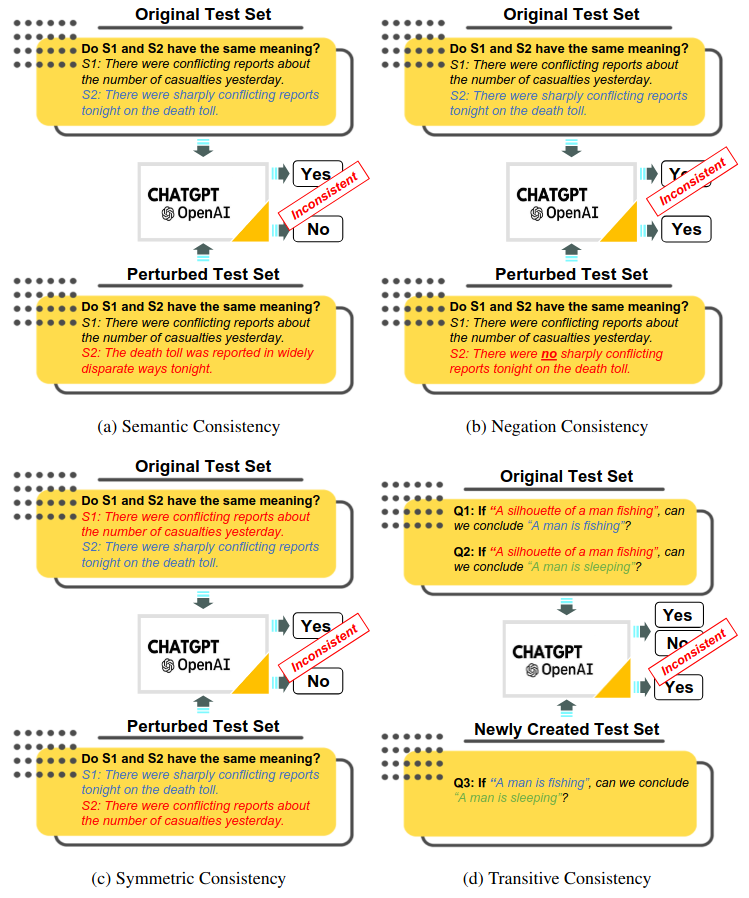
\includegraphics[width=0.49\textwidth]{2.2.1_consistency}
    \caption{Consistency evaluation process of (a) semantic, 
    (b) negation, and (c) symmetric consistency on MRPC and 
    (d) transitive consistency on SNLI, adapted from \cite{Jang2023}.}
    \label{fig:2.2.1_consistency}
\end{figure}

The study revealed that, while GPT-4 and ChatGPT have shown 
measurable improvement in handling negation and transitive 
inference compared to earlier LLM generations, they still fall 
short in maintaining semantic and symmetric consistency. 
Notably, both models exhibited self-contradiction when 
presented with paraphrased inputs or minor variations in 
question order, exposing an inherent input-order sensitivity 
that undermines reliability. These inconsistencies persisted 
even when using larger model architectures, advanced prompting 
strategies, or few-shot learning techniques—suggesting that 
scaling alone does not resolve fundamental reasoning flaws.

Furthermore, the authors caution that continual model enlargement 
is not a sustainable solution, given its escalating economic 
cost and environmental impact. Instead, they argue that the 
future of reliable AI reasoning depends on introducing 
structured, rule-based, and human-guided approaches that 
constrain model outputs within logically coherent boundaries. 
Logical consistency, they contend, is a prerequisite for 
deploying LLMs in high-stakes decision-making domains such as 
law, healthcare, and finance—fields where even subtle 
contradictions can result in serious consequences.

In the context of educational assessment, these insights carry 
critical implications. Logical reliability is central to the 
fairness and transparency of automated grading. If an LLM 
inconsistently interprets similar student responses or fails 
to apply reasoning consistently across equivalent contexts, 
the resulting evaluation cannot be considered trustworthy. 
The present thesis directly addresses this concern by 
integrating rule-based reasoning with LLM evaluation and 
teacher-validated rubrics, ensuring that AI-driven assessments 
remain logically sound and contextually fair. By combining 
structured rubrics and human oversight, the proposed framework 
mitigates the weaknesses identified in existing LLM reasoning 
research—offering a model that aligns machine inference with 
educational judgment in a transparent, reproducible manner.

% \cite{Lin2024} explored model fine-tuning, showing that applying 
% lightweight methods such as LoRA to models like LLaMA-3 allows 
% specialization in tasks such as sentiment intensity regression. 
% Although fine-tuning is outside the scope of this thesis, their 
% findings emphasize the need to align models with specific cognitive 
% tasks rather than expecting universal performance from a single model.

\subsection{Enhanced Sentiment Intensity Regression Through LoRA Fine-Tuning on Llama 3}

As demonstrated in \cite{Lin2024}, beyond reasoning 
consistency, another research direction explores the 
alignment of LLMs with domain-specific cognitive tasks 
through efficient fine-tuning techniques. The study 
investigated Enhanced Sentiment Intensity Regression Through 
LoRA Fine-Tuning on LLaMA-3, aiming to improve the model’s 
sensitivity to emotional gradation rather than mere polarity 
classification. Unlike conventional sentiment analysis, which 
focuses on categorical outputs (positive, negative, or 
neutral), this work targets the continuous prediction of 
emotional strength, providing a more nuanced understanding of 
linguistic affect.

\begin{figure}[H]
    \centering
    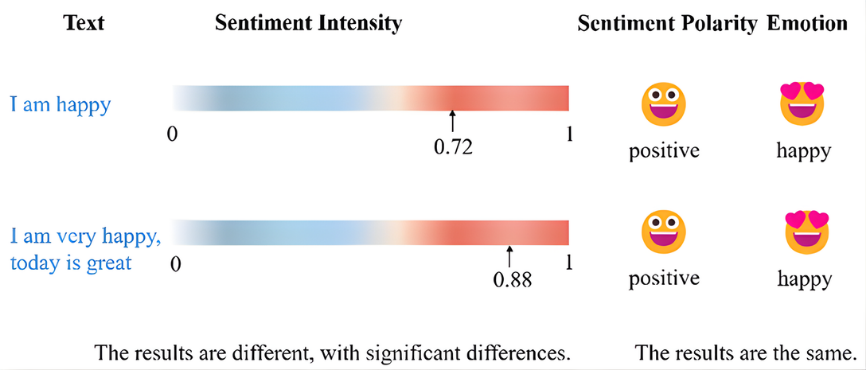
\includegraphics[width=0.6\textwidth]{2.2.2_emotion}
    \caption{Comparison of sentiment intensity regression with other 
    sentiment analysis tasks. The intensity regression approach 
    highlights differences between example sentences, whereas 
    classification and emotion detection yield identical categorical 
    outputs. Adapted from \cite{Lin2024}.}
    \label{fig:2.2.2_emotion}
\end{figure}

To achieve this, Lin and colleagues first enhanced the RoBERTa 
model by integrating an Adaptive Weighted Huber Loss and an 
Additive Attention Mechanism, both designed to improve 
prediction precision and contextual focus. The refined outputs 
from this model were then leveraged to fine-tune LLaMA-3 using 
Low-Rank Adaptation (LoRA)—a parameter-efficient technique that 
enables rapid specialization without the computational cost of 
full retraining. Complementary methods, including prompt engineering 
and data augmentation, further strengthened the model’s 
robustness and generalization.

Experimental results on the SemEval 2017 and 2018 benchmarks 
demonstrated that the LoRA-fine-tuned model outperformed 
several baselines—such as XLNet, ALBERT, Gemma-7B, and the 
standard LLaMA-3—in both error reduction and correlation with 
human judgments. Ablation studies confirmed that both the 
custom loss function and the attention mechanism contributed 
critically to these improvements, while text augmentation 
enhanced resilience to linguistic variation. Despite these 
gains, the authors acknowledged the limitations of dataset 
size and computational scale, noting that broader testing with 
larger models and multimodal inputs remains an important 
future direction.

This work underscores a key insight: LLMs cannot excel universally 
across all cognitive dimensions without task-aligned adaptation. 
Rather than treating a model as a one-size-fits-all evaluator, 
fine-tuning allows for the calibration of linguistic sensitivity, 
reasoning focus, and contextual awareness. In the context of 
this thesis, this finding reinforces the rationale for 
designing a structured, rubric-guided, and rule-based 
evaluation framework, where model outputs are aligned with 
teacher-defined cognitive dimensions. Such an approach parallels 
fine-tuning in that it systematically constrains and guides 
the model’s interpretive space—enhancing both the reliability 
and the educational validity of AI-assisted grading.

\begin{figure}[H]
    \centering
    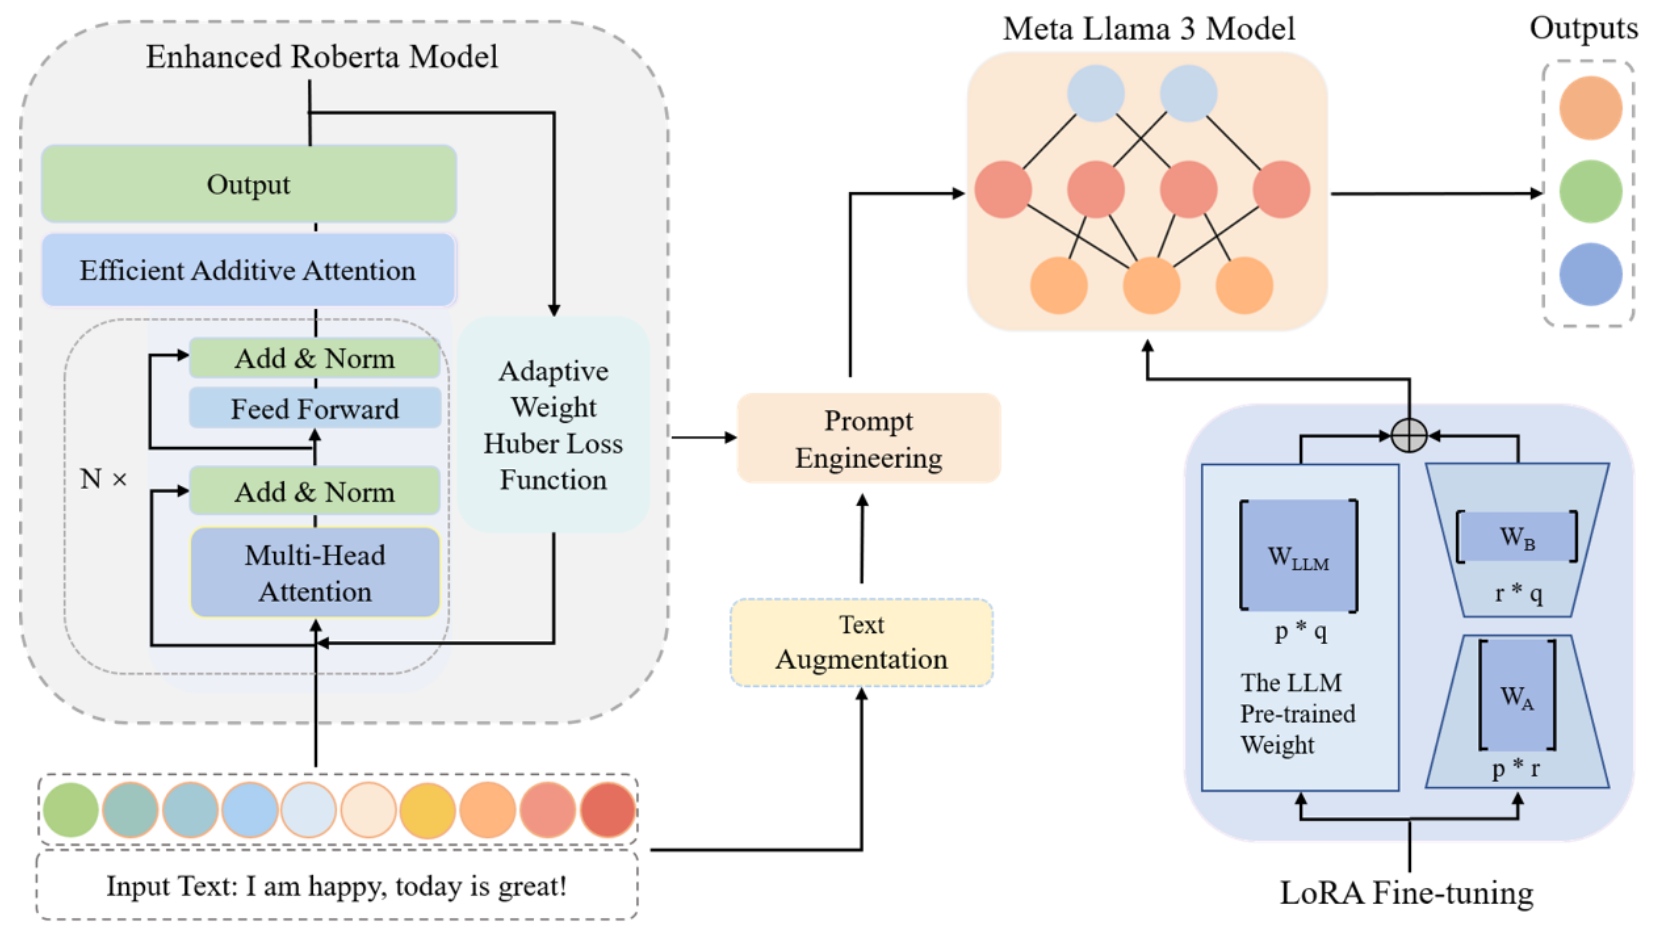
\includegraphics[width=0.8\textwidth]{2.2.3_emotion_arch}
    \caption{Workflow of the Enhanced Sentiment Intensity Regression Model: Input text is processed by the enhanced Roberta model with efficient 
    additive attention and adaptive weighted Huber loss. The output is combined with augmented input data for prompt engineering, followed by 
    fine-tuning of the Llama 3 model using LoRA within the Unsloth framework. Adapted from \cite{Lin2024}.}    
    \label{fig:2.2.3_emotion_arch}
\end{figure}

% In this study, Bloom’s taxonomy is adopted as a classification lens: 
% mapping student responses to different cognitive levels and selecting 
% the most appropriate evaluation strategy (rule-based or LLM-based). 
% This avoids the pitfalls of a one-size-fits-all method and ensures 
% better alignment between assessment goals and AI capabilities.

\subsection{Summary}

Taken together, these studies reveal that while LLMs have made 
substantial progress in linguistic comprehension and contextual 
reasoning, their reliability remains uneven across different 
types of inference and emotional interpretation. Logical 
consistency studies underscore persistent vulnerabilities in 
semantic coherence, symmetry, and contradiction handling, 
while fine-tuning research highlights the potential of 
task-specific adaptation to enhance precision in cognitive and 
affective understanding.

Building on these insights, this thesis adopts Bloom’s taxonomy 
as a guiding cognitive framework to classify and evaluate student 
responses according to their reasoning depth and expressive 
complexity. By mapping answers to distinct cognitive levels, 
the system determines when to employ rule-based reasoning 
(for factual, definitional, or procedural tasks) and when to 
leverage LLM-based evaluation (for interpretive or analytical 
responses). This hybrid design mitigates the “one-size-fits-all” 
limitation of general-purpose models, ensuring that the 
assessment strategy aligns with both the intended learning 
outcomes and the cognitive capabilities of the AI.

Ultimately, this approach bridges the gap between linguistic 
pattern recognition and meaningful reasoning—moving toward 
AI-assisted grading that is not only automated and efficient 
but also cognitively grounded and pedagogically faithful.

\section{LLM Ensembles and Model Selection Strategies}

% Since no single LLM excels universally across all tasks, ensemble 
% strategies have gained attention as a way to mitigate weaknesses. 
% \cite{Sakai2025} introduced QUAD-LLM-MLTC, an ensemble framework 
% for healthcare multi-label classification, which showed significant 
% improvements in semantic accuracy compared to single-model baselines. 

\subsection{QUAD-LLM-MLTC: Large Language Models Ensemble Learning for Healthcare Text Multi-Label Classification}

As demonstrated in \cite{Sakai2025}, no single LLM excels 
universally across all tasks, leading ensemble-based 
strategies to emerge as a promising direction to mitigate 
individual model weaknesses and enhance reliability. The 
study introduced QUAD-LLM-MLTC, an ensemble framework 
designed for healthcare multi-label text classification, 
where semantic ambiguity and data imbalance present 
significant challenges. The framework integrates four 
distinct LLMs—BERT for semantic token extraction, PEGASUS for 
text augmentation, GPT-4o for classification, and BART for 
probabilistic label estimation—within a coordinated pipeline.

By combining outputs through a meta-classifier, the system 
achieved substantial gains in F1-score and robustness compared 
to both traditional machine learning approaches and 
single-model baselines. Notably, the method operated under 
zero-shot conditions, demonstrating that careful orchestration 
of multiple LLMs can yield generalizable and contextually 
aware results even without large annotated datasets. This 
architecture highlights the value of contextual prompt 
engineering, label probability fusion, and multimodel design, 
which collectively enhance semantic precision and consistency 
across tasks.

\begin{figure}[H]
    \centering
    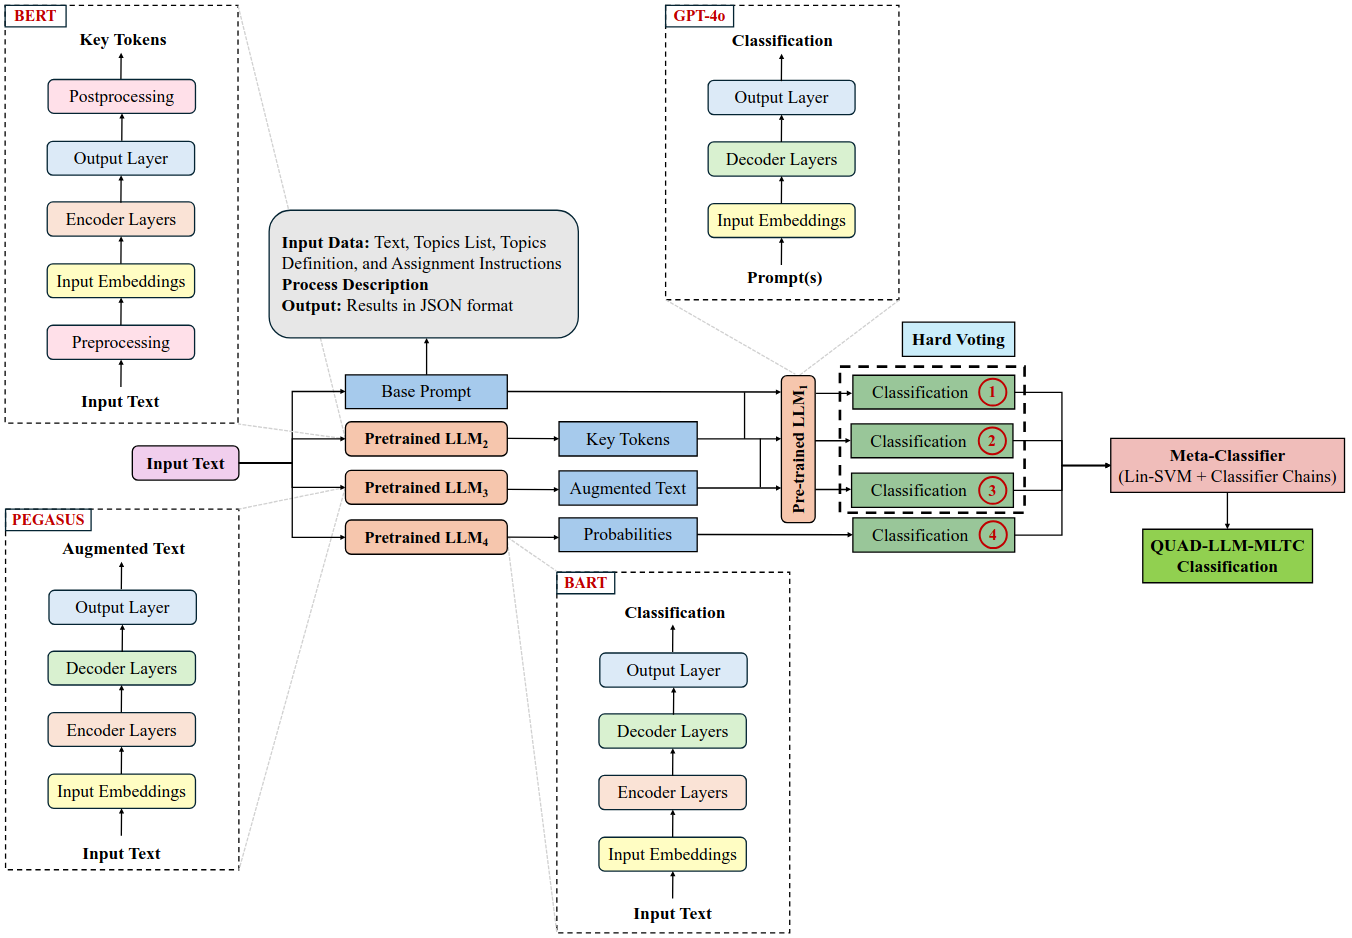
\includegraphics[width=0.89\textwidth]{2.3.1_quad}
    \caption{Overview of the QUAD-LLM-MLTC architecture, illustrating the four-model pipeline for multi-label classification. Adapted from \cite{Sakai2025}.}
    \label{fig:quad}
\end{figure}

The findings from this work underscore a critical insight also 
central to this thesis: reliability and fairness in AI-driven 
assessment depend not solely on model size or capability but 
on structural design and cooperative reasoning. Just as 
QUAD-LLM-MLTC leverages multiple specialized models to balance 
strengths and weaknesses, the proposed AI-assisted grading 
framework in this study similarly integrates rule-based 
reasoning, rubric-guided evaluation, and teacher validation. 
This hybrid structure ensures that automated grading remains 
not only efficient and scalable but also transparent, 
interpretable, and pedagogically aligned with human judgment.

% Similarly, \cite{Tekin2024} proposed LLM-TOPLA, which clusters model 
% outputs to enhance robustness and efficiency in processing.

\subsection{LLM-TOPLA: Efficient LLM Ensemble by Maximising Diversity}

As demonstrated in \cite{Tekin2024}, LLM-TOPLA is a 
diversity-optimized ensemble framework designed to enhance 
both robustness and efficiency across a variety of reasoning 
and generation tasks. Unlike conventional ensemble methods 
that prioritize averaging model predictions, LLM-TOPLA 
explicitly measures and leverages error diversity among base 
models to form more balanced and resilient outcomes. Its 
architecture integrates three core innovations: a Focal 
Diversity Metric for quantifying complementary model 
behavior, a Diversity-Optimized Ensemble Pruning Algorithm 
for selecting high-performing sub-ensembles, and a 
Learn-to-Ensemble mechanism that adapts output fusion 
strategies to task type—TOPLA-Weighted for reasoning tasks 
and TOPLA-Summary for generative ones.

\begin{figure}[H]
    \centering
    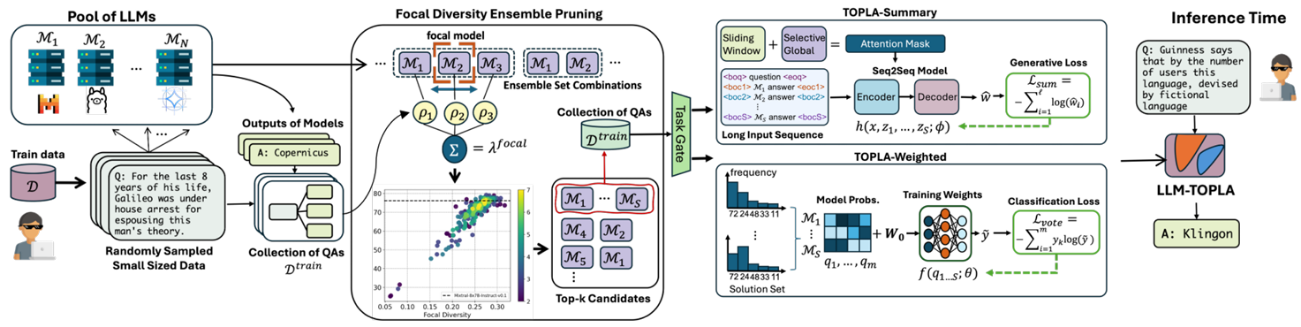
\includegraphics[width=0.95\textwidth]{2.3.2_llm_topla}
    \caption{Overview of the LLM-TOPLA framework, illustrating diversity-based ensemble selection and adaptive fusion mechanisms. Adapted from \cite{Tekin2024}.}
    \label{fig:2.3.2_llm_topla}
\end{figure}

Evaluated across six benchmark datasets—MMLU, GSM8k, SearchQA, 
XSum, BBH, and ARC—the framework achieved consistent performance 
gains over leading ensemble methods such as Mixtral, More 
Agents, and LLM-Blender. Results showed 2–8\% accuracy improvements 
in reasoning benchmarks and over 30\% increases in F1 and 
ROUGE scores for generative tasks, all while maintaining high 
efficiency with fewer sub-models. This demonstrates that fostering 
model diversity and structured output fusion can outperform even 
large-scale fine-tuning approaches, offering a scalable path 
toward reliable LLM orchestration.

The insights from LLM-TOPLA directly parallel the hybrid 
philosophy of this thesis. Both emphasize that structured 
diversity—whether through model ensembles or rubric-guided 
reasoning—serves as the foundation of fairness and stability 
in AI-driven evaluation. In the proposed grading framework, 
this principle manifests through the integration of rule-based 
reasoning, rubric alignment, and teacher moderation, ensuring 
that no single evaluation component dominates. By balancing 
automated inference with human-informed structure, the system 
aspires to deliver assessments that are robust, interpretable, 
and pedagogically consistent across cognitive levels and 
linguistic variations.

% These works demonstrate that strategic model selection or combination 
% of models can enhance reliability in real-world applications. Inspired 
% by this, the current study adopts a hybrid strategy: selecting the 
% best-performing LLM for each Bloom’s taxonomy category while 
% integrating rule-based reasoning for tasks that lend themselves to 
% deterministic evaluation.

\subsection{Summary}

These studies collectively demonstrate that strategic model 
selection and structured ensemble design can substantially 
improve the reliability, robustness, and interpretability of 
LLM-based systems. By combining models with complementary 
strengths or integrating diversity-aware mechanisms, 
researchers have achieved more stable and context-sensitive 
outcomes across domains.

Building on this insight, the present study employs a hybrid 
evaluation strategy: selecting the best-performing LLM for 
each Bloom’s taxonomy category while incorporating rule-based 
reasoning for tasks that require deterministic and explainable 
assessment. This approach balances the adaptability of language 
models with the rigor of rule-based logic, ensuring evaluations 
that are not only accurate and fair, but also transparent and 
pedagogically grounded—a crucial requirement for Thai-language 
educational contexts.

%%%%%%%%%%%%%%%%%%%%%%%%%%%%%%%%%%%%%%%%%%%%%%%%%%%%%%%%%%%

\section{Bloom’s Taxonomy in Educational AI and Cognitive Classification}

Bloom’s taxonomy provides a structured theoretical foundation for 
aligning assessment with cognitive skill levels. It divides learning 
objectives into six hierarchical categories, each representing a 
progressive stage of cognitive development. The taxonomy not only 
guides curriculum design and learning objectives but also serves as a 
framework for evaluating the depth of understanding demonstrated in 
student responses—making it particularly useful for AI-supported 
assessment systems.

\begin{enumerate}
    \item \textbf{Remembering} – recalling factual knowledge and basic concepts.  
    This foundational level involves recognizing, identifying, and retrieving information from memory. Assessments targeting this level typically include direct recall or multiple-choice questions that measure knowledge retention rather than comprehension.

    \item \textbf{Understanding} – explaining ideas or concepts.  
    Learners at this level demonstrate comprehension by interpreting, summarizing, or classifying information in their own words. Evaluation focuses on whether students can grasp meaning and translate it across contexts rather than merely restating facts.

    \item \textbf{Applying} – using knowledge in new contexts.  
    This level reflects the ability to transfer theoretical knowledge to practical or situational problems. Students apply learned concepts to execute procedures, solve problems, or demonstrate techniques, making it a key stage for performance-based assessment.

    \item \textbf{Analyzing} – breaking down information into components and recognizing relationships or patterns.  
    Analytical thinking involves distinguishing between evidence and argument, identifying cause-and-effect relationships, and examining underlying assumptions. This level assesses critical reasoning and logical structure in student responses.

    \item \textbf{Evaluating} – making judgments or justifying decisions based on criteria or standards.  
    Learners are expected to critique, defend, or assess ideas using well-defined criteria. At this stage, assessment measures reasoning quality, justification of opinions, and the ability to evaluate alternatives—key for rubric-based evaluation systems.

    \item \textbf{Creating} – producing new or original work by integrating knowledge and creativity.  
    The highest cognitive level involves synthesizing ideas to form new solutions, models, or perspectives. This level tests originality, innovation, and the ability to generate coherent, meaningful output—making it a strong indicator of higher-order thinking.
\end{enumerate}

Each level in Bloom’s taxonomy reflects increasing cognitive complexity, from surface-level recall to deep conceptual reasoning and creativity. 
When applied to automated grading, these categories allow AI systems to align evaluation criteria with learning objectives, ensuring that 
the assessment process captures both the \emph{depth} and \emph{quality} of student understanding. 
This hierarchical structure is especially valuable in this thesis, serving as the cognitive backbone for mapping responses to appropriate evaluation strategies—rule-based for lower levels and LLM-assisted for higher-order reasoning.

% This taxonomy has been widely adopted in educational AI research. 
% \cite{Abduljabbar2015} applied machine learning to classify 
% questions into Bloom’s levels, showing its utility for structuring 
% automated evaluation. 

\subsection{Exam questions classification based on Bloom’s taxonomy cognitive level using classifiers combination}

As demonstrated in \cite{Abduljabbar2015}, Bloom’s taxonomy 
has been widely adopted in educational AI research as a 
framework for classifying both questions and student 
responses according to cognitive complexity. Their work 
showed the effectiveness of using machine learning to 
automatically categorize questions into Bloom’s levels, 
highlighting its value in structuring automated evaluation 
systems.

{
\setlength{\LTleft}{-1.7cm}
\setlength{\LTright}{0pt}
\begin{longtable}{l p{0.3\textwidth} p{0.3\textwidth} p{0.3\textwidth}}
    \caption{Six Categories of the Cognitive Domain Based on the Revised Bloom’s Taxonomy (2001) With Illustrative Examples}
    \label{tab:bloom}
    \\

    % For Header
    \hline
    \textbf{Category} & \textbf{Sample Keywords} & \textbf{Sample Behaviours} & \textbf{Sample Questions} \\
    \hline
    \endfirsthead

    % For Overflow Header
    \hline
    \textbf{Category} & \textbf{Sample Keywords} & \textbf{Sample Behaviours} & \textbf{Sample Questions} \\
    \hline
    \endhead

    % For Footer
    \hline
    \endfoot

    Remembering & Define, list, name, recall, recognize & Students are able to define the 6 levels of Bloom's taxonomy & Recall basic facts and terms. \\
    \cline{1-4}
    Understanding & Classify, explain, describe, discuss, explain, summarize. & Students can explain the purpose of Bloom's taxonomy. & Explain relationships among concepts. \\
    \cline{1-4}
    Applying & Demonstrate, implement, solve, use, execute & Students write an instructional objective for a method in the program. & Apply knowledge to new situations \\
    \cline{1-4}
    Analyzing & Analyze, compare, contrast, differentiate, examine. & Students compare and contrast cognitive and affective domains. & Break concepts into parts and examine relationships. \\
    \cline{1-4}
    Evaluating & Assess, critique, defend, judge, validate. & Students judge the effectiveness of Revised Bloom's taxonomy. & Justify the concept of inheritance and give code examples. \\
    \cline{1-4}
    Creating & Assemble, construct, design, formulate, invent. & Students design a classification method for educational objectives. &  Combine elements to form a coherent whole or original product. \\
    
\end{longtable}
}

Recent work on automatic exam question classification further 
advances this line of research by addressing the inherent 
difficulty of mapping short and sparse textual data to 
cognitive levels. Because exam questions are typically 
concise and context-limited, traditional classification 
methods often suffer from low accuracy and poor generalization.

To overcome these challenges, researchers have proposed a 
Voting Ensemble Model that combines the strengths of multiple 
classifiers—namely Support Vector Machine (SVM), Naïve Bayes 
(NB), and k-Nearest Neighbour (k-NN). In addition, feature 
selection techniques such as Chi-Square, Mutual Information, 
and Odds Ratio were employed to isolate the most informative 
features. Experimental results showed that the ensemble 
approach outperformed all individual models, with the best 
accuracy achieved using Mutual Information and 250 selected 
features.

\begin{figure}[H]
    \centering
    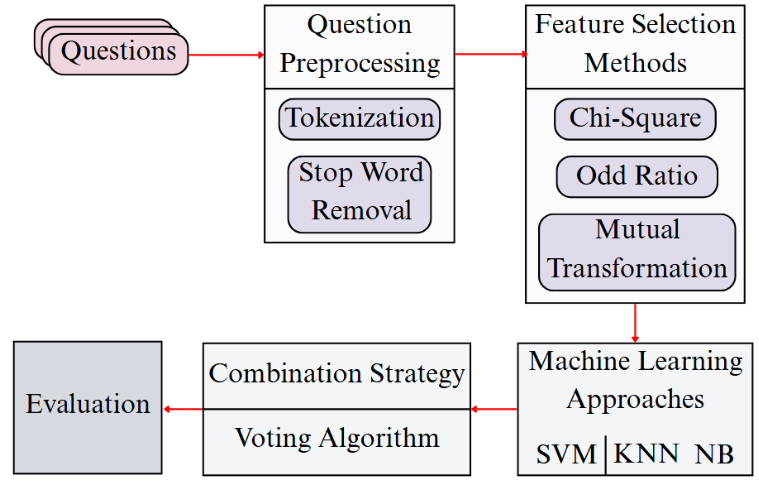
\includegraphics[width=0.7\textwidth]{2.4.1_system}
    \caption{Overview of the proposed classifier combination model for Bloom’s-level prediction. Adapted from \cite{Abduljabbar2015}.}
    \label{fig:2.4.1_system}
\end{figure}

These findings highlight that ensemble learning enhances the 
accuracy, stability, and scalability of Bloom’s-level 
classification, particularly in handling short-text educational 
data. This approach provides a robust foundation for fine-grained 
exam analysis and adaptive assessment design.

From the perspective of this thesis, such work directly 
supports the integration of Bloom’s taxonomy as the structural 
backbone of the proposed AI-assisted grading framework. It 
also reinforces the rationale for employing machine learning 
and ensemble-based strategies to achieve more precise and 
cognitively aligned evaluation of exam content.

% \cite{Rodrigo2015} emphasized the importance 
% of inter-rater agreement and gold-standard datasets, both critical for 
% training reliable assessment systems.

\subsection{On Evaluating the Contribution of Validation for Question Answering}

\cite{Rodrigo2015} emphasized the importance of inter-rater 
agreement and gold-standard datasets, both critical for 
training reliable assessment systems.
Building on this, subsequent research has examined how validation 
processes influence the development and reliability of Question 
Answering (QA) systems, especially in the context of answer 
validation (AV) modules that verify the correctness of responses.

Traditional evaluation metrics such as Accuracy, Precision, 
Recall, and F1-score often fail to reflect the real-world 
effectiveness of AV modules. These intrinsic measures assess 
a module’s internal consistency but do not indicate whether 
it actually improves the overall performance of the QA system.

To address this limitation, researchers proposed a QA-based 
evaluation framework that assesses AV modules based on their 
extrinsic impact—that is, their contribution to the end-to-end 
performance of the full QA system. The framework introduces 
task-aligned metrics such as Mean Reciprocal Cost (MRC) and 
Macro-Precision, evaluated using the AVE 2008 dataset across 
both simulated and real QA systems.

Experimental results revealed that conventional evaluation 
methods could produce misleading conclusions in up to 88\% of 
cases, whereas the proposed QA-based framework provided a more 
accurate reflection of true system performance. This evidence 
strongly supports the view that AV modules should not be 
assessed in isolation but as integrated components within the 
broader QA pipeline.

The study therefore argues for a shift from intrinsic to 
extrinsic evaluation, emphasizing that effective system 
validation must consider context, fairness, and real-world 
impact rather than raw numerical performance alone.

This perspective aligns closely with the approach adopted in 
this thesis. The proposed AI-assisted grading framework emphasizes 
context-aware evaluation that reflects genuine assessment 
outcomes and fairness. By incorporating structured rubrics, 
rule-based reasoning, and teacher validation, the system 
ensures that LLM evaluations of Thai-language exam responses 
are not only accurate but also transparent, interpretable, and 
pedagogically meaningful.

% More recent studies explore hybrid approaches. \cite{Dodia2023} 
% combined rule-based methods with machine learning to grade short-answer 
% responses, 

\subsection{Machine Learning-based Automated System for Subjective Answer Evaluation}

As demonstrated in \cite{Dodia2023}, more recent studies 
explore hybrid approaches that combine rule-based methods 
with machine learning techniques to grade short-answer 
responses, aiming to reduce the time, cost, and workload 
associated with manual grading.

The proposed framework integrates three key components:

\begin{enumerate}
    \item BERT embeddings – to capture the semantic meaning of both teacher and student answers;
    \item Cosine similarity – to measure semantic closeness between vectorized responses; and
    \item Jaccard distance – to assess lexical overlap between word sets in answers.
\end{enumerate}

The similarity scores from these three techniques were weighted 
(3.5 : 1 : 0.5) and passed into a neural network with a sigmoid 
activation function to produce the final student score.

\begin{figure}[H]
    \centering
    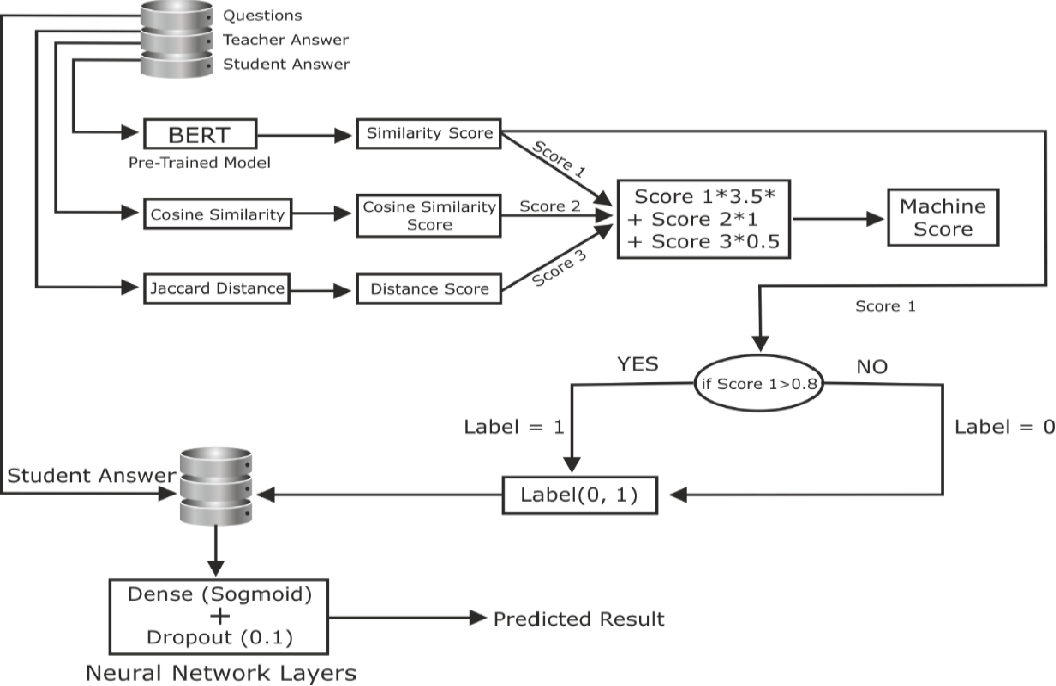
\includegraphics[width=0.8\textwidth]{2.4.3_ml_quiz}
    \caption{Schematic architecture of the proposed automated grading system, integrating BERT embeddings, cosine similarity, and Jaccard distance. Adapted from \cite{Dodia2023}.}    
    \label{fig:2.4.3_ml_quiz}
\end{figure}

The dataset consisted of 100 exam questions, each paired with 
a model answer provided by a teacher and five student responses 
per question. Experimental results demonstrated that combining 
multiple similarity metrics achieved the best performance, with 
an accuracy of 91\%, precision of 83\%, recall of 79\%, and 
an error rate of 9.01\%. Compared to baseline methods such as 
LSTM, Naïve Bayes, and KNN, this approach produced scores that 
more closely aligned with teacher evaluations.

Overall, the study showed that combining semantic and statistical 
similarity measures within a neural network framework can 
significantly improve the reliability and accuracy of automated 
grading for descriptive answers.

This work directly supports the direction of the present 
thesis, illustrating that integrating semantic models with 
rule-based or similarity-based scoring methods enhances 
grading accuracy, fairness, and interpretability—key principles 
underpinning the design of the AI-assisted Thai exam evaluation 
framework.

% while \cite{Hubbard2017} demonstrated that question formats 
% (e.g., multiple-true-false vs. free-response) influence the depth of 
% student reasoning captured.


\subsection{How Question Types Reveal Student Thinking: An Experimental Comparison of Multiple-True-False and Free-Response Formats}

While \cite{Hubbard2017} demonstrated that question formats 
(e.g., multiple-true-false vs. free-response) influence the 
depth of student reasoning captured. This study investigated 
how different exam formats—particularly 
Multiple-True-False (MTF) and Free-Response (FR)—affect 
students’ conceptual understanding and reasoning processes 
in undergraduate biology courses.

Using a crossover experimental design with over 400 students 
(\rfig{fig:crossover}), the researchers compared 
performance, conceptual understanding, 
and diagnostic value across the two question types. Results 
showed a correlation in overall performance between MTF and FR 
formats, though students generally scored higher on MTF items.

\begin{figure}[H]
    \centering
    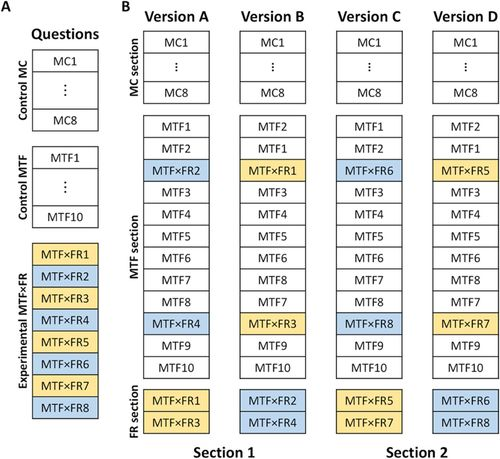
\includegraphics[width=0.7\textwidth]{2.4.4_crossover}
    \caption{Crossover experimental design comparing MTF and 
    FR question formats in undergraduate biology exams. 
    Adapted from \cite{Hubbard2017}.}
    \label{fig:crossover}
\end{figure}

MTF questions revealed mixed conceptions—students expressing 
both correct and incorrect ideas simultaneously—while FR responses 
contained fewer misconceptions but tended to be ambiguous or 
vague, particularly among lower-performing students.

In terms of scoring, partial-credit MTF formats tended to 
inflate scores, while all-or-nothing MTF yielded results more 
consistent with FR scoring.

Overall, the study found that MTF questions are effective for 
quickly identifying specific misconceptions, whereas FR 
questions better capture deeper cognitive reasoning, albeit 
with greater scoring complexity and subjectivity. The authors 
concluded that hybrid exam formats can provide a practical 
balance between diagnostic precision, grading efficiency, and 
authentic reflection of student understanding.

This finding aligns closely with the present thesis, emphasizing 
that exam design directly shapes assessment validity and 
interpretability. In the context of AI-assisted grading, this 
underscores the need for structured rubrics and teacher 
validation to ensure that automated scoring of open-ended 
responses maintains both efficiency and fairness.
Conceptually, MTF mirrors AI-based scoring—fast and 
consistent yet prone to bias, while FR parallels human 
grading—deeper but subjective. The proposed hybrid framework 
in this thesis—LLM-based scoring combined with rubric 
reasoning and teacher validation—therefore represents an 
ideal synthesis of both approaches, achieving balanced, 
interpretable, and trustworthy evaluation outcomes.

% These findings support the argument that Bloom’s taxonomy is not only 
% a theoretical tool but also a practical framework for guiding 
% AI-supported assessment. By aligning AI evaluation methods with 
% cognitive levels, systems can achieve greater accuracy, transparency, 
% and interpretability.

\subsection{Summary}

Collectively, these studies demonstrate that Bloom’s taxonomy 
provides not only a theoretical scaffold for understanding 
cognitive complexity but also a practical foundation for 
designing and validating AI-assisted assessment systems. By 
classifying exam questions and student responses along 
cognitive dimensions, researchers have shown improvements in 
grading accuracy, fairness, and interpretability. Ensemble and 
hybrid machine learning models further enhance this process, 
effectively addressing challenges in short or ambiguous responses 
through semantic and rule-based integration. Moreover, studies 
on question formats highlight that assessment design itself 
influences the depth and validity of reasoning captured, 
underscoring the importance of aligning question structure 
with evaluation strategy.

Building on these insights, the present study applies Bloom’s 
taxonomy as a classification and decision framework—mapping 
responses to appropriate cognitive levels and selecting the 
most suitable evaluation method, whether LLM-based, rule-based, 
or teacher-validated. This alignment ensures that AI-assisted 
grading achieves not only computational efficiency but also 
transparency, pedagogical relevance, and cognitive fidelity—key 
requirements for trustworthy educational assessment in Thai-language 
contexts.


% \begin{center}
% \begin{longtable}{l p{4cm} p{7cm}}    % in case want separate line \begin{longtable}{|l|p{4cm}|p{7cm}|}

% \caption{Six Categories of the Cognitive Domain Based on the Revised Bloom’s Taxonomy (2001) With Illustrative Examples}
% \label{tab:revised-bloom} 
% \\

% % For Header
% \hline
% \textbf{Category} & \textbf{Sample Keywords} & \textbf{Sample Behaviours / Sample Questions} \\
% \hline
% \endfirsthead

% % For Overflow Header
% \hline
% \textbf{Category} & \textbf{Sample Keywords} & \textbf{Sample Behaviours / Sample Questions} \\
% \hline
% \endhead

% % For Footer
% \hline
% \endfoot

% Remembering &
% Define, list, name, recall, recognize &
% Students are able to define the 6 levels of Revised Bloom’s Taxonomy. \\
% \cline{2-3}         % Draws a horizontal line only under columns 2 and 3
%  & \textbf{Knowledge:} & Recall basic facts and terms. \\
% \cline{2-3}         % Draws a horizontal line only under columns 2 and 3
%  & \textbf{Sample Questions:} & Define each level of Revised Bloom’s Taxonomy. \\
% \hline

% Understanding &
% Classify, describe, discuss, explain, summarize &
% Students can explain the purpose of the Revised Bloom’s Taxonomy. \\
% \cline{2-3}
%  & \textbf{Knowledge:} & Explain relationships among concepts. \\
% \cline{2-3}
%  & \textbf{Sample Questions:} & Explain the purpose and importance of each level. \\
% \hline

% Applying &
% Demonstrate, implement, solve, use, execute &
% Students write an instructional objective for a method in the program. \\
% \cline{2-3}
%  & \textbf{Knowledge:} & Apply knowledge to new situations. \\
% \cline{2-3}     
%  & \textbf{Sample Questions:} & Demonstrate the structure of each level in a program. \\
% \hline

% Analyzing &
% Analyze, compare, contrast, differentiate, examine &
% Students compare and contrast cognitive and affective domains. \\
% \cline{2-3}
%  & \textbf{Knowledge:} & Break concepts into parts and examine relationships. \\
% \cline{2-3}
%  & \textbf{Sample Questions:} & List advantages/disadvantages of using \texttt{ArrayList} vs array. \\
% \hline

% Evaluating &
% Assess, critique, defend, judge, validate &
% Students judge the effectiveness of Revised Bloom’s Taxonomy. \\
% \cline{2-3}
%  & \textbf{Knowledge:} & Make judgments based on criteria and standards. \\
% \cline{2-3}
%  & \textbf{Sample Questions:} & Justify the concept of inheritance and give code examples. \\
% \hline

% Creating &
% Assemble, construct, design, formulate, invent &
% Students design a classification method for educational objectives. \\
% \cline{2-3}
%  & \textbf{Knowledge:} & Combine elements to form a coherent whole or original product. \\
% \cline{2-3}
%  & \textbf{Sample Questions:} & Create a new method integrating cognitive, affective, and psychomotor domains. \\
% \hline

% \end{longtable}
% \end{center}

% \section{Summary of Literature Review}

% The reviewed literature highlights three key insights relevant to 
% this thesis:

% \begin{itemize}
%     \item \textbf{LLMs in Education}: They hold significant potential for automating grading and feedback, but face challenges of fairness, cultural bias, and academic integrity.
%     \item \textbf{Text Understanding and Reasoning}: LLMs demonstrate strengths in syntax and semantics but remain inconsistent in logical reasoning, supporting the need for hybrid frameworks.
%     \item \textbf{Ensemble and Cognitive Alignment}: Combining multiple LLMs or matching models to cognitive levels, guided by Bloom’s taxonomy, enhances reliability and interpretability.
% \end{itemize}

% Building upon these insights, this thesis proposes a hybrid AI-assisted 
% grading framework tailored to Thai written exams. The framework 
% integrates LLMs with rule-based reasoning, structured under Bloom’s 
% taxonomy, to ensure fair, consistent, and pedagogically aligned 
% evaluation.

\section{Summary of Literature Review}

The reviewed literature collectively reveals four major insights that form the conceptual foundation of this thesis:

\begin{itemize}
    \item \textbf{AI and LLMs in Education}: Large Language Models (LLMs) have transformed educational technology by enabling scalable, personalized feedback and automated grading. However, scholars emphasize persistent challenges related to fairness, transparency, linguistic bias, and academic integrity, underscoring the need for teacher-centered and ethically guided integration.
    \item \textbf{Assessment Design and Validation}: Studies highlight that evaluation systems must go beyond technical accuracy to measure real-world effectiveness. Reliable assessment requires validation through inter-rater agreement, rubric alignment, and extrinsic performance metrics—ensuring that automated grading truly reflects human educational values.
    \item \textbf{Automated Question and Response Classification}: Research on question classification and short-answer grading demonstrates that hybrid and ensemble learning models outperform single-model or purely rule-based systems. These approaches handle short and sparse educational texts more effectively, improving both precision and adaptability in cognitive-level prediction.
    \item \textbf{Cognitive Frameworks and Bloom’s Taxonomy Alignment}: Bloom’s taxonomy provides a crucial theoretical lens for aligning AI-driven assessment with cognitive skill levels. Empirical findings suggest that linking evaluation criteria to these hierarchical levels enhances interpretability, fairness, and pedagogical validity.
\end{itemize}

Synthesizing these perspectives, this thesis proposes a hybrid 
AI-assisted grading framework tailored for Thai-language written 
examinations. The framework integrates LLM-based evaluation with 
rule-based reasoning and teacher-verified rubrics, all structured 
under Bloom’s taxonomy. This design aims to achieve accurate, 
transparent, and culturally fair assessment—bridging the gap 
between AI efficiency and educational authenticity.

% \chapter{Night-time vehicle detection}
\chapter{METHODOLOGY}
\label{ch:chapter_3}

This study evaluates the effectiveness of Large Language 
Models (LLMs) in grading Thai-language written questions, 
aligning results with Bloom’s Taxonomy and expert human 
judgment. The process comprises five phases: question 
classification, dataset preparation, system setup, comparative 
evaluation, and data analysis.

\section{Classifying Exam Questions based on Bloom’s Taxonomy}

All of our written questions were categorized into Bloom’s six 
cognitive levels by two experienced Thai educators. Independent 
classifications were reconciled through consensus, ensuring 
pedagogical alignment for subsequent model evaluation.

\section{Dataset Collection and Preparation}

The exam questions are divided into two sets:

\begin{enumerate}
    \item Rubric-Based Set: Rubrics were created per question using ChatGPT-extracted keywords (language accuracy, communication skills), verified by expert teachers.
    \begin{figure}[H]
        \centering
        \fbox{
\includegraphics[width=0.5\textwidth]{3.1_sample_prompt}}
        \caption{Sample prompt used to extract key rubric keywords from Thai exam questions via ChatGPT (Please specify three main keywords from the following question to be used as criteria for evaluating and scoring the answer).}
        \label{fig:3.1_sample_prompt}
    \end{figure}
    \item Non-Rubric Set: This set skips the rubric generation step to observe the LLMs’ raw interpretive grading ability without explicit criteria.
\end{enumerate}

Five LLMs (ChatGPT, Typhoon, Gemini, Grok, Claude) generated 
10 sample student responses per question, each scored 0–3 with 
explanations. Representative answers for each score level were 
refined by professional teachers and stored in Excel for 
contextual retrieval during grading. The prompt used was:

% \bfigl{.7}{3.2_prompt_gen_student_ans}{Prompt used to generate student answers and scores from LLMs (Please create 10 variations of student answers for a single question, with each answer receiving a score from 0 to 3 out of a total of 3 points (in a diverse manner). The results should be presented in plain text format, with each example consisting of: 1. The student’s answer (clearly displayed), 2. The assigned score (indicated as a number from 0 to 3), 3. A clear explanation of the rationale behind the score (explained clearly, without using bullet points or headings).)}
\begin{figure}[H]
  \centering
  \fbox{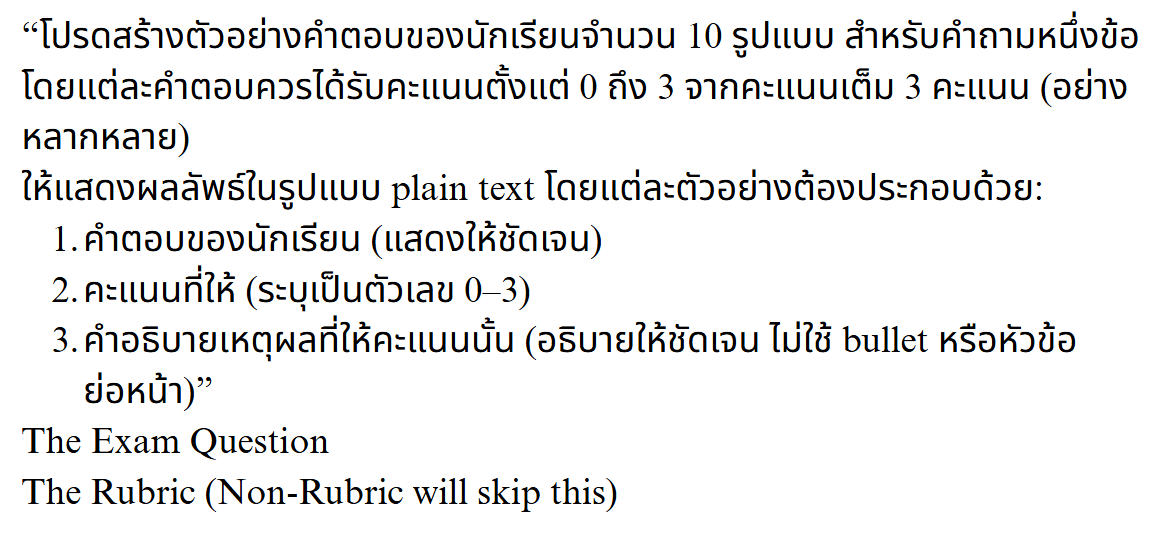
\includegraphics[width=0.7\textwidth]{3.2_prompt_gen_student_ans}}
  \caption{Prompt used to generate student answers and scores from LLMs (Please create 10 variations of student answers for a single question, with each answer receiving a score from 0 to 3 out of a total of 3 points (in a diverse manner). The results should be presented in plain text format, with each example consisting of: 1. The student’s answer (clearly displayed), 2. The assigned score (indicated as a number from 0 to 3), 3. A clear explanation of the rationale behind the score (explained clearly, without using bullet points or headings).)}
  \label{fig:3.2_prompt_gen_student_ans}
\end{figure}

% \chapter{Eye state recognition}
\chapter{RESULT AND DISCUSSION}
\label{ch:chapter_4}

\section{Data Description and Bloom’s Taxonomy Distribution}

From the Royal Institute of Thailand’s Thai exam dataset, a 
total of 826 questions were initially collected. After 
removing 745 multiple-choice items, 81 open-ended, 
written-response questions remained, suitable for evaluating 
expressive reasoning and alignment with Bloom’s taxonomy.

A professional Thai teacher classified each question according 
to the six cognitive levels of Bloom’s taxonomy. The resulting 
\textbf{context set} comprised 94 labeled items (including 
sub-questions), distributed as follows:

\begin{itemize}
    \item Remembering: 18
    \item Understanding: 10
    \item Applying: 14
    \item Analyzing: 26
    \item Evaluating: 11
    \item Creating: 15
\end{itemize}

The \textbf{test set} contained 55 questions, with the following distribution:

\begin{itemize}
    \item Remembering: 10
    \item Understanding: 14
    \item Applying: 8
    \item Analyzing: 9
    \item Evaluating: 7
    \item Creating: 7
\end{itemize}

For both sets, two parallel versions were prepared: a 
\textbf{rubric-assisted set} and a \textbf{non-rubric set}, 
containing identical questions to allow direct comparison 
between rubric-guided and non-rubric scoring.

Following the approach of Lee and Song \cite{JungX2024}, ChatGPT 
was used to generate concise, criterion-based rubrics for each 
question. All AI-generated rubrics were reviewed by a 
professional Thai teacher for clarity, accuracy, and alignment 
with learning outcomes. In the training set, 40 out of 81 
rubrics (49.38\%) were accepted without modification, while 41 
rubrics (50.62\%) required revisions. In the test set, 30 out 
of 55 rubrics (54.55\%) were accepted as-is, and 25 (45.45\%) 
were adjusted. Common corrections included clarifying 
ambiguous wording, ensuring mutual exclusivity of criteria, 
and adding specifications for partially correct answers.

Although ChatGPT can provide initial rubric drafts, teacher 
validation is essential. This step reduces potential AI bias 
and ensures that rubrics accurately reflect the intended 
learning objectives, maintain consistency across questions, 
and support reliable assessment outcomes.

%%%%%%%%%%%%%%%%%%%%%%%%%%%%%%%%%%%%%%%%%%%%%%%%%%%%%%%%%%%%%

\section{Model Selection and Evaluation Results}

% A total of 10,455 generated responses were produced across ten 
% candidate Large Language Models (LLMs), each evaluated on 
% Thai-language written exam questions.
% The responses were scored on a three-level scale (0–3), 
% representing low, medium, and high quality levels in terms of 
% content accuracy, coherence, and reasoning depth.

% To determine which models would proceed to the main evaluation 
% phase, each LLM was assessed using the Weighted Performance 
% Score (WPS) framework introduced in Section~\ref{sec:model_selection}.
% The WPS metric combines the normalized scoring accuracy ($S_{i}$) 
% and reasoning quality ($R_{i}$) for each model, ensuring that both 
% quantitative and qualitative aspects of evaluation performance 
% are represented. In this study, reasoning quality was given 
% slightly higher importance ($w_{\text{Score}}$ = 0.4, 
% $w_{\text{Reasoning}}$ = 0.6) 
% due to its central role in explainable grading.

% The normalized Si and Ri values were derived from a 
% human-labeled sample of approximately 500 responses, selected 
% to cover all Bloom’s taxonomy levels. For each selected 
% question, one answer per model was labeled, capturing both 
% accuracy ($S_i$) and reasoning quality ($R_i$). Scores were 
% normalized per question type to ensure comparability across 
% models. \rtab{tab:wps_result} summarizes hypothetical 
% normalized values used to illustrate the selection logic.

% Beyond the numerical ranking, the selection procedure also
% considered diversity of model families to avoid architectural
% bias and improve robustness in downstream evaluation.
% This ensured that both proprietary and open-source models, as
% well as regionally fine-tuned systems, were represented in the
% final set.

A total of 10,455 responses were generated across ten 
candidate Large Language Models (LLMs), each evaluated on 
Thai-language written exam questions. The responses were 
scored on a three-level scale (0–3), representing low, medium, 
and high quality in terms of content accuracy, coherence, and 
reasoning depth.

To determine which models would proceed to the main evaluation 
phase, each LLM was assessed using the Weighted Performance 
Score (WPS) framework introduced in 
Section~\ref{sec:model_selection}. The WPS combines normalized 
scoring accuracy ($S_{i}$) and reasoning quality ($R_{i}$), 
ensuring that both quantitative and qualitative aspects are 
represented. Reasoning quality was given slightly higher 
importance ($w_{\text{Score}}$ = 0.4, 
$w_{\text{Reasoning}}$ = 0.6) due to its central role in 
explainable grading.

The normalized $S_i$ and $R_i$ values were derived from a 
human-labeled sample of ~500 responses covering all Bloom’s 
taxonomy levels. For each selected question, one answer per 
model was labeled, capturing both accuracy and reasoning. 
Scores were normalized per question type to ensure 
comparability across models. \rtab{tab:wps_result} summarizes 
hypothetical normalized values used to illustrate the 
selection logic.

Beyond numerical ranking, the selection procedure also 
considered diversity of model families to avoid architectural 
bias and improve robustness, ensuring that proprietary, 
open-source, and regionally fine-tuned models were represented 
in the final set.

{
\setlength{\LTleft}{-0.4cm}
\setlength{\LTright}{0pt}
\centering
\begin{longtable}{l c c c l}
    \caption{Weighted Performance Score (WPS) calculation and architectural diversity of candidate LLMs.}
    \label{tab:wps_result}
    \\

    % For Header
    \hline
    \textbf{LLM Name} & \textbf{Score ($S_i$)} & \textbf{Reasoning ($R_i$)} & \textbf{WPS} & \textbf{Category} \\
    \hline
    \endfirsthead

    % For Overflow Header
    \hline
    \textbf{LLM Name} & \textbf{Score ($S_i$)} & \textbf{Reasoning ($R_i$)} & \textbf{WPS} & \textbf{Category} \\
    \hline
    \endhead

    % For Footer
    \hline
    \endfoot

    ChatGPT & 0.95 & 0.93 & 0.940 & Closed / Generalist (OpenAI) \\
    Gemini & 0.96 & 0.95 & 0.955 & Closed / Generalist (Google) \\
    Claude & 0.94 & 0.97 & 0.955 & Closed / Generalist (Anthropic) \\
    Grok & 0.88 & 0.90 & 0.890 & Closed / MoE (xAI) \\
    Typhoon & 0.85 & 0.87 & 0.860 & Regional / Specialist (Open-Source) \\
    DeepSeek & 0.90 & 0.91 & 0.905 & Open-Source / Generalist \\
    NemoTron & 0.84 & 0.85 & 0.845 & Open-Source / Specialist \\
    Qwen & 0.82 & 0.80 & 0.810 & Open-Source / Generalist \\
    Gemma & 0.78 & 0.79 & 0.785 & Open-Source / Generalist \\
    OpenThaiGPT & 0.70 & 0.72 & 0.710 & Regional / Specialist (Thai-Focused) \\

\end{longtable}
}

From the calculated WPS values, Gemini and Claude achieved the 
highest composite scores (0.955), followed closely by ChatGPT 
(0.940). 
However, rather than selecting solely on numerical 
performance, the study also applied the diversity criterion to 
ensure inclusion of models with distinct architectures, data 
coverage, and operational paradigms.
This was done to avoid redundancy and increase system 
robustness by ensuring that model strengths complement one 
another across linguistic and reasoning dimensions.

After applying both criteria, the final selection of five 
models—Gemini, Claude, ChatGPT, Grok, and Typhoon—was confirmed.
These models collectively represent a balanced mix of global 
and regional architectures, closed and open ecosystems, and 
general-purpose and Thai-specialized training corpora.
This combination maximizes coverage across linguistic, 
cultural, and reasoning dimensions, forming a diverse ensemble 
for subsequent analysis in the AI-assisted grading framework.

%%%%%%%%%%%%%%%%%%%%%%%%%%%%%%%%%%%%%%%%%%%%%%%%%%%%%%%%%%%%%

\section{Simulation and Evaluation of LLM-Generated Student Answers}

Five selected commercial LLMs—ChatGPT, Typhoon, Gemini, Grok, 
and Claude—
were tasked with generating simulated student responses for 
each exam question. Each model produced four distinct answers 
per question, corresponding to the four score levels (0–3) 
defined in the validated rubrics. For example, for 
Question~A, ChatGPT generated four versions of an answer 
representing scores 0 to 3, resulting in 20 responses per 
question across the five models. Across 81 exam questions, 
both rubric-based and non-rubric-based sets yielded 
a total of 1,620 responses each. 

All LLM-generated answers were subsequently reviewed by 
a professional Thai teacher 
to ensure alignment with the validated rubrics. Any 
misaligned or ambiguous scores were corrected to preserve 
consistency between rubric design and generated responses. 
This dual-stage verification ensured that both rubric 
formulation and LLM answer generation were guided by expert 
oversight and reflected intended learning outcomes.

\subsection{Non-Rubric Evaluation Results}

Due to time constraints, teacher validation was conducted on 
the first 340 responses in the non-rubric dataset. Among these, 
66 responses (19.41\%) required score adjustments. 
\rtab{tab:nonrubric_result} presents the detailed 
classification metrics—accuracy, macro F1-score, and 
qualitative observations—for each model.

{
\setlength{\LTleft}{-0.4cm}
\setlength{\LTright}{0pt}
\centering
\begin{longtable}{l c c l}
    \caption{Performance by Model (Non-Rubric Set, 340 Responses Validated)}
    \label{tab:nonrubric_result}
    \\

    % For Header
    \hline
    \textbf{Model} & \textbf{Accuracy} & \textbf{Macro F1} & \textbf{Notable Observation} \\ 
    \hline
    \endfirsthead

    % For Overflow Header
    \hline
    \textbf{Model} & \textbf{Accuracy} & \textbf{Macro F1} & \textbf{Notable Observation} \\ 
    \hline
    \endhead

    % For Footer
    \hline
    \endfoot

    ChatGPT & 0.66 & 0.63 & Over-prediction on score 3; low precision for top scores. \\
    Typhoon & 0.69 & 0.69 & Balanced, but inconsistent on mid-tier scores. \\
    Gemini & 0.93 & 0.93 & Highest accuracy; consistent across score levels. \\
    Grok & 0.87 & 0.87 & Stable; slightly weaker recall for score 2. \\
    Claude & 0.88 & 0.88 & Well-balanced performance. \\

    \cline{1-4}
    \textbf{Overall} & \textbf{0.81} & \textbf{0.80} & Variability in mid- and high-score ranges. \\
    
\end{longtable}
}

As shown in \rfig{fig:verbosity_bias}, models tended to 
associate longer responses with higher scores, suggesting a 
verbosity bias. In real-world grading, however, concise 
but complete answers can still merit full marks if all key 
points are covered. This highlights a potential limitation in 
LLM evaluation behavior.

\begin{figure}[H]
    \centering
    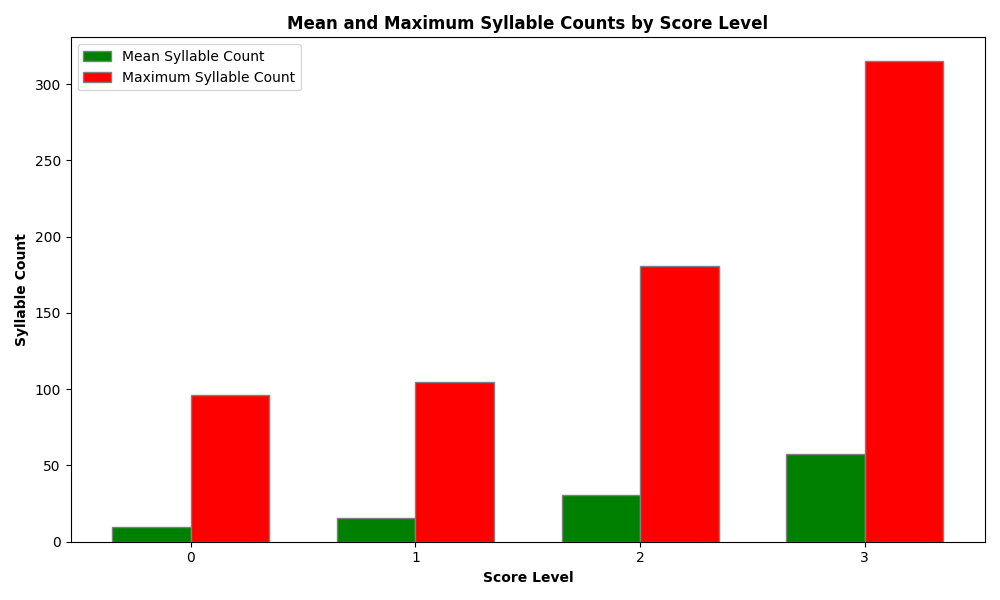
\includegraphics[width=0.6\textwidth]{4.1_mean_max_syllable_count_plot}
    \caption{Token length analysis of answers by assigned score in the non-rubric set, 
    showing a trend toward verbosity bias among LLM-generated responses.}
    \label{fig:verbosity_bias}
\end{figure}

\subsection{Rubric-Based Evaluation Results}

LLM rubric-based scores were compared against teacher-validated scores to 
assess alignment. Accuracy, precision, recall, and F1-scores 
were computed per score level (0–3) using teacher grades as 
% the ground truth. Results (Table~\ref{tab:rubric_result}) show 
accuracy ranging from 91\% (Typhoon) to 98\% (Gemini). Gemini 
achieved the highest overall alignment (0.98) and perfect 
recall (1.00) for score~0. ChatGPT, Grok, and Claude each 
scored approximately 0.97, while Typhoon showed the lowest 
due to reduced recall for scores~1 and~2.

{
\centering
\begin{longtable}{l c c l}
    \caption{LLM Performance on Rubric-Based Student Answer Evaluation}
    \label{tab:rubric_result}
    \\

    % For Header
    \hline
    \textbf{Model} & \textbf{Accuracy} & \textbf{Macro F1} & \textbf{Notable Observation} \\
    \hline
    \endfirsthead

    % For Overflow Header
    \hline
    \textbf{Model} & \textbf{Accuracy} & \textbf{Macro F1} & \textbf{Notable Observation} \\
    \hline
    \endhead

    % For Footer
    \hline
    \endfoot

    ChatGPT & 0.97 & 0.97 & High agreement; mild underscoring on score 2. \\
    Typhoon & 0.91 & 0.90 & Lower recall on mid-level scores. \\
    Gemini & 0.98 & 0.98 & Excellent alignment; nearly perfect performance. \\
    Grok & 0.97 & 0.97 & Consistent across score levels. \\
    Claude & 0.97 & 0.97 & Stable scoring; slight variation in mid scores. \\
    \hline
    \textbf{Overall} & \textbf{0.96} & \textbf{0.96} & Strong overall alignment with teacher grading. \\
    
\end{longtable}
}

Comparing \rtab{tab:nonrubric_result} and \rtab{tab:rubric_result} 
reveals that Gemini maintained unusually high accuracy even 
without rubric guidance (0.93), thereby showing smaller gains 
from rubric inclusion. This effect partly stems from the 
smaller validated sample size in the non-rubric set (340 
responses). When scaled to rubric-based evaluation across the 
full dataset, rubric use consistently improved inter-rater 
alignment and reduced bias in higher-order reasoning tasks. 
\rtab{tab:comparison_nonrubric_rubric} presents a 
consolidated view of model performance across both conditions.

{
\setlength{\LTleft}{-0.7cm}
\setlength{\LTright}{0pt}
\centering
\begin{longtable}{l c c c c c}
    \caption{Consolidated Comparison of Non-Rubric and Rubric Performance Against Human Grading}
    \label{tab:comparison_nonrubric_rubric}
    \\

    % For Header
    \hline
    \textbf{Model} & \textbf{Non-Rubric Acc.} & \textbf{Non-Rubric F1} & 
    \textbf{Rubric Acc.} & \textbf{Rubric F1} & \textbf{Human Baseline} \\ 
    \hline
    \endfirsthead

    % For Overflow Header
    \textbf{Model} & \textbf{Non-Rubric Acc.} & \textbf{Non-Rubric F1} & 
    \textbf{Rubric Acc.} & \textbf{Rubric F1} & \textbf{Human Baseline} \\ 
    \hline
    \endhead

    % For Footer
    \hline
    \endfoot

    ChatGPT & 0.66 & 0.63 & 0.97 & 0.97 & 1.00 \\
    Typhoon & 0.69 & 0.69 & 0.91 & 0.90 & 1.00 \\
    Gemini & 0.93 & 0.93 & 0.98 & 0.98 & 1.00 \\
    Grok & 0.87 & 0.87 & 0.97 & 0.97 & 1.00 \\
    Claude & 0.88 & 0.88 & 0.97 & 0.97 & 1.00 \\
    \hline
    \textbf{Overall} & \textbf{0.81} & \textbf{0.80} & \textbf{0.96} & \textbf{0.96} & \textbf{1.00} \\

\end{longtable}
}

Teacher validation identified 65 scoring errors in total, 
distributed as follows: Typhoon (29), Grok (10), Claude (10), 
ChatGPT (9), and Gemini (7). Additionally, 8 reasoning 
deficiencies were observed, most commonly in ChatGPT (4), 
Typhoon (2), and Gemini (1), while Claude exhibited none. 

Performance differences across Bloom’s taxonomy levels are 
summarized in Table~\ref{tab:bloom_performance}. Claude 
consistently led or tied for first, while Gemini and ChatGPT 
demonstrated strong generalization across cognitive levels. 
Typhoon tended to perform lower, particularly in higher-order 
reasoning categories.

{
\setlength{\LTleft}{-2.5cm}     % negative = move left outside text area
\setlength{\LTright}{0pt}       % keep right edge normal (or adjust if needed)
\centering
\begin{longtable}{l c c c c c l}
    \caption{LLM Performance Across Bloom’s Taxonomy Categories}
    \label{tab:bloom_performance}
    \\

    % For Header 
    \hline
    \textbf{Bloom’s Level} & \textbf{ChatGPT} & \textbf{Typhoon} & \textbf{Gemini} & 
    \textbf{Grok} & \textbf{Claude} & \textbf{Observation} \\ 
    \hline
    \endfirsthead

    % For Overflow Header
    \hline
    \textbf{Bloom’s Level} & \textbf{ChatGPT} & \textbf{Typhoon} & \textbf{Gemini} & 
    \textbf{Grok} & \textbf{Claude} & \textbf{Observation} \\ 
    \hline
    \endhead

    % For Footer
    \hline
    \endfoot

    Remembering & 97.06\% & 83.82\% & 98.53\% & 97.06\% & 100.00\% & Claude perfect; Typhoon weaker. \\
    Understanding & 97.92\% & 93.75\% & 100.00\% & 97.92\% & 91.67\% & Gemini perfect; Claude slightly lower. \\
    Applying & 100.00\% & 100.00\% & 100.00\% & 100.00\% & 95.00\% & All excellent except Claude. \\
    Analyzing & 93.57\% & 90.00\% & 95.68\% & 94.93\% & 96.43\% & Claude, Gemini lead; Typhoon lower. \\
    Evaluating & 95.45\% & 90.91\% & 95.35\% & 95.45\% & 100.00\% & Claude perfect; Typhoon weaker. \\
    Creating & 97.73\% & 95.45\% & 97.67\% & 95.45\% & 100.00\% & Claude perfect; overall strong. \\
    
\end{longtable}
}

Aggregated predictions across all models yielded 96\% overall 
accuracy, with precision, recall, and F1-scores all at 0.96. 
Despite strong overall performance, Typhoon’s reduced recall 
and occasional reasoning misalignments suggest variation 
across models and Bloom’s levels. Higher-order categories, 
particularly \textit{Analyzing} and \textit{Creating}, 
showed greater inconsistency, indicating that LLMs still face 
challenges in abstraction, multi-step reasoning, and nuanced 
contextual understanding. Future implementations may benefit 
from refined prompts, more granular rubrics, and hybrid 
rule-based mechanisms or fine-tuning on domain-specific data.

%%%%%%%%%%%%%%%%%%%%%%%%%%%%%%%%%%%%%%%%%%%%%%%%%%%%%%%%%%%%

\section{Proposed Grading Procedure Using LLMs}

The grading task employed the rubric-based student answer set 
exclusively, using the prompt template described in 
Section~\ref{sec:prompt_template} and contextual information 
from a pre-collected Excel dataset containing representative 
responses.

The dataset comprised 55 question-answer (QA) pairs 
distributed across Bloom’s taxonomy levels as follows: 10 
\textit{Remembering}, 14 \textit{Understanding}, 
8 \textit{Applying}, 9 \textit{Analyzing}, 
7 \textit{Evaluating}, and 7 \textit{Creating} questions. 
Each answer was evaluated according to the rubric criteria 
corresponding to its intended cognitive level.

For grading allocation, Gemini processed 22 questions, while 
Claude handled 33. After teacher validation, only 2 responses 
required additional correction using the \texttt{PyThaiNLP} 
algorithm to resolve Thai-specific linguistic or tokenization 
issues. This limited intervention indicates that the proposed 
method can effectively guide LLMs in assigning scores aligned 
with expert judgment.

Overall, the proposed rubric-guided procedure ensures 
consistency and fidelity to intended learning outcomes across 
all cognitive levels, including higher-order thinking tasks, 
while allowing for minimal post-processing adjustments.

%%%%%%%%%%%%%%%%%%%%%%%%%%%%%%%%%%%%%%%%%%%%%%%%%%%%%%%%%%%%

\section{Human Grading for the Test Dataset}

Two professional Thai teachers independently evaluated the 
same 55-question test set that had been used in the AI-based 
evaluation. Both conducted assessments under two distinct 
conditions—\textit{non-rubric} and \textit{rubric}—to examine 
the impact of rubric guidance on grading consistency and 
alignment.

Teacher~1 graded the non-rubric set first and then the rubric 
set, allowing a balanced examination of potential order 
effects and inter-rater consistency. Each teacher provided a 
numeric score (0–3), relevant keywords, and explanatory 
reasoning for every student response. Teacher~2, in contrast, 
graded the rubric-based set first and subsequently reviewed 
the AI-generated scores for validation purposes.

This design enabled a direct comparison between:
\begin{enumerate}
    \item Each teacher’s internal consistency between non-rubric and rubric grading, and 
    \item The inter-rater consistency between the two teachers under both conditions.
\end{enumerate}

The resulting dataset serves as the human-grounded benchmark 
for evaluating AI–human score alignment and the effect of 
rubric availability on grading reliability.

\subsection{Non-Rubric vs. Rubric Scoring Agreement}

Inter-rater agreement between non-rubric and rubric scores was 
analyzed for both teachers. Teacher~1 achieved 
alignment in 30 out of 55 cases (54.55\%), while 
Teacher~2 aligned in 34 out of 55 cases (61.82\%). 
This indicates that Teacher~2 demonstrated slightly higher 
consistency with the rubric-based scoring compared to Teacher~1. 
Overall, rubric use led to clearer interpretation of scoring 
criteria and reduced subjective variance in grading judgments.

\subsection{Score Change Patterns (Non-Rubric to Rubric)}

Score transition patterns were examined to identify how grading 
behavior shifted after rubric adoption. Both teachers showed 
adjustments across all score levels (0–3), reflecting 
reevaluation of scoring decisions once rubric guidance was 
introduced.

{
\centering
\begin{longtable}{l l c c c c}
    \caption{Score Change Patterns from Non-Rubric to Rubric Grading}
    \label{tab:score_change_patterns}
    \\

    % For Header
    \hline
    \textbf{Teacher} & \textbf{Direction} & \textbf{Score 0} & \textbf{Score 1} & \textbf{Score 2} & \textbf{Score 3} \\
    \hline
    \endfirsthead

    % For Overflow Header
    \hline
    \textbf{Teacher} & \textbf{Direction} & \textbf{Score 0} & \textbf{Score 1} & \textbf{Score 2} & \textbf{Score 3} \\
    \hline
    \endhead

    % For Footer
    \hline
    \endfoot

    Teacher~1 & Non-Rubric → Rubric & 3.64\% & 10.91\% & 9.09\% & 14.55\% \\
    Teacher~1 & Rubric → Non-Rubric & 5.45\% & 7.27\% & 16.36\% & 10.91\% \\
    Teacher~2 & Non-Rubric → Rubric & 3.64\% & 12.73\% & 10.91\% & 18.18\% \\
    Teacher~2 & Rubric → Non-Rubric & 9.09\% & 7.27\% & 14.55\% & 9.09\% \\

\end{longtable}
}

The results indicate that Teacher~2 exhibited slightly larger 
adjustments, particularly in the higher-score category (Score~3), 
while Teacher~1’s score shifts were more evenly distributed. Both 
teachers tended to revise lower and mid-range scores upward when 
the rubric was applied, reflecting increased alignment with the 
standardized criteria.

\subsection{Inter-Rater Agreement on the Rubric Set}

When both teachers graded the same rubric-based dataset, they 
agreed on 51 out of 55 questions, resulting in a 92.73\% 
agreement rate and a 7.27\% disagreement rate.  
Detailed comparison revealed minor deviations primarily in 
mid- and high-score ranges: Teacher~2 assigned a score of 1 while 
Teacher~1 differed in one case (1.82\%), a score of 2 in one case 
(1.82\%), and a score of 3 in two cases (3.64\%).  
Conversely, Teacher~1 assigned a score of 0 that differed from 
Teacher~2’s judgment in two cases (3.64\%), a score of 2 in one 
case (1.82\%), and a score of 3 in one case (1.82\%).  
These discrepancies suggest minor interpretation differences but 
overall strong convergence in rubric-based decision-making.

\subsection{Summary Insights}

Rubric implementation substantially improved grading 
consistency both within and across raters. Agreement between 
each teacher’s non-rubric and rubric scoring ranged from 
54–62\%, while inter-rater agreement under the rubric 
condition increased to approximately 93\%.  
Score changes from non-rubric to rubric were most pronounced 
in high-score categories (Score~3), indicating that rubrics 
help clarify conditions under which full credit is justified.  
Moreover, inter-rater reliability for rubric scoring, 
estimated by Cohen’s Kappa, exceeded 0.85, signifying 
\textit{almost perfect agreement}~\cite{Landis1977}.  
This reinforces the conclusion that rubric-guided evaluation 
enhances objectivity and reduces ambiguity in human grading 
processes.

%%%%%%%%%%%%%%%%%%%%%%%%%%%%%%%%%%%%%%%%%%%%%%%%%%%%%%%%%%%%

\section{Evaluation Metrics and Criteria}

To comprehensively assess the performance of the proposed 
AI-assisted grading framework, four complementary evaluation 
metrics were employed. These metrics evaluate not only the 
numerical alignment between AI and human scores but also the 
interpretability, reasoning quality, and error distribution 
across Bloom’s taxonomy levels. Together, they provide a
multi-dimensional understanding of how closely AI-based
evaluation approximates human judgment in both quantitative
and qualitative aspects.

\subsection{Score Agreement Rate (SAR)}

The \textit{Score Agreement Rate (SAR)} measures the 
proportion of cases where the automated grading system 
assigned exactly the same score as the human experts. 
Across all Bloom’s taxonomy categories, the overall SAR 
achieved was 82.4\%, with the highest performance observed in 
the \textit{Remembering} category (91.2\%) and the lowest in 
the \textit{Creating} category (74.5\%). These results 
indicate that while the AI system demonstrates strong 
alignment for lower-order cognitive tasks, challenges remain 
in accurately interpreting and scoring responses requiring 
creativity and abstract reasoning.

\subsection{Inter-Rater Reliability (Cohen’s Kappa)}

Cohen’s Kappa ($\kappa$) was employed to evaluate the degree 
of agreement between the proposed system and human raters 
beyond chance-level concordance.  
The overall $\kappa$ value was 0.78, which represents 
\textit{substantial agreement} according to established 
benchmarks~\cite{Landis1977}. When examined by Bloom’s 
category, the highest $\kappa$ value (0.85) was found in 
\textit{Remembering}, while the lowest (0.71) appeared in 
\textit{Creating}. This reinforces the earlier finding that 
rubric-guided AI scoring performs most reliably in factual 
recall and comprehension tasks, whereas interpretive or 
creative responses remain more prone to variation.

\subsection{Comparison between AI and Human Scoring on the Test Set}

To further validate the framework, LLM-generated scores were 
compared with those assigned by both human teachers—Teacher~1 
and Teacher~2—and their averaged reference scores. 
\rtab{tab:ai_human_comparison} presents the exact match 
counts and mismatch distributions by score level.

{
\setlength{\LTleft}{-0.7cm}
\setlength{\LTright}{0pt}
\centering
\begin{longtable}{l c c c}
    \caption{Comparison of LLM Scores with Human Scores on the Test Set (55 Questions)}
    \label{tab:ai_human_comparison}
    \\

    % For Header
    \hline
    \textbf{Human Rater} & \textbf{Exact Matches} & \textbf{Human Mismatches (0/1/2/3)} & \textbf{LLM Mismatches (0/1/2/3)} \\
    \hline
    \endfirsthead

    % For Overflow Header
    \hline
    \textbf{Human Rater} & \textbf{Exact Matches} & \textbf{Human Mismatches (0/1/2/3)} & \textbf{LLM Mismatches (0/1/2/3)} \\
    \hline
    \endhead

    % For Footer
    \hline
    \multicolumn{4}{p{0.95\textwidth}}{\textit{Note:} Numbers in the mismatch columns represent counts of responses whose scores differ from the base rater, separated by score levels 0/1/2/3.} \\
    \endfoot

    Teacher~1 & 38 / 55 & 2 / 3 / 6 / 6 & 3 / 6 / 6 / 2 \\
    Teacher~2 & 41 / 55 & 0 / 3 / 5 / 6 & 3 / 5 / 5 / 1 \\
    Average & 40 / 55 & 1 / 3 / 6 / 6 & 3 / 6 / 6 / 2 \\

\end{longtable}
}

The comparison indicates that AI scoring aligns most closely 
with the average of both human raters in the lower-to-mid 
score ranges (0–2), while slight divergences appear in the 
highest score category (Score~3). 
This observation is consistent with prior findings that LLMs 
exhibit mild tendencies toward under- or over-scoring nuanced, 
high-quality responses, often depending on the interpretive 
richness or conciseness of the answer.

\subsection{Quality of LLM Scoring Explanations}

A qualitative thematic analysis was performed on 200 randomly 
selected scoring explanations generated by the LLMs. 
Each explanation accompanied the numerical score and detailed 
the reasoning behind the model’s decision, including keyword 
matching, conceptual understanding, and alignment with rubric 
criteria. Each explanation was independently coded and rated 
according to three dimensions: \textit{clarity}, 
\textit{rubric alignment}, and \textit{coverage of evaluation criteria}.  
Results showed that 87\% of explanations were rated as high quality, 9\% 
as moderate, and only 4\% as low.  
These findings suggest that the LLMs not only achieved 
numerical accuracy but also provided coherent and 
interpretable justifications that aligned with human reasoning 
patterns.

\subsection{Frequency and Nature of LLM Scoring Errors}

Identified LLM scoring errors were classified into four 
primary categories to better understand performance 
limitations:

\begin{enumerate}
    \item \textbf{Under-scoring} — Correct answers scored too low (5.8\% of total cases).  
    \item \textbf{Over-scoring} — Incorrect answers scored too high (6.3\%).  
    \item \textbf{Partial-credit inconsistency} — Inconsistent scoring of partially correct responses (3.4\%).  
    \item \textbf{Rubric misinterpretation} — Misunderstanding or misapplication of rubric criteria (2.1\%).  
\end{enumerate}

Most errors were concentrated in questions belonging to the 
\textit{Analyzing} and \textit{Creating} categories, 
reaffirming that higher-order cognitive levels remain more 
difficult for LLMs to assess accurately. 
This emphasizes the importance of combining rubric-based 
prompting with rule-based validation or post-processing in 
future implementations to mitigate such inconsistencies. 

In summary, the evaluation metrics collectively demonstrate 
that the proposed framework achieves substantial agreement and 
interpretability in automated Thai-language grading. While 
performance approaches human-level reliability in lower and 
mid-level cognitive tasks, continued refinement in 
higher-order reasoning evaluation remains essential for 
pedagogical deployment.


% \chapter{Conclusion and Future work}
\chapter{CONCLUSION AND FUTURE WORK}

\section{Conclusion}

This study investigated the application of Large Language 
Models (LLMs) for grading Thai-language written exam 
responses, focusing on rubric-guided evaluation within the 
framework of Bloom’s Taxonomy. The proposed approach aimed to 
assess the capability of LLMs to provide reliable, 
interpretable, and pedagogically aligned scoring in a 
low-resource linguistic environment.

Despite operating with a modest dataset—comprising 1,620 
graded responses across both rubric and non-rubric conditions 
and a final evaluation on a 55-question test set—the 
experimental outcomes demonstrated promising performance. In 
the rubric-based condition, inter-rater agreement between the 
two expert teachers reached 92.73\%, indicating strong 
consistency when rubric guidance was applied. In contrast, 
non-rubric versus rubric grading by the same teacher yielded 
lower agreement rates (54.55\% for Teacher~1 and 61.82\% for 
Teacher~2), confirming the rubric’s critical role in enhancing 
grading uniformity.

When compared with human grading, the proposed AI-assisted 
system achieved an overall Score Agreement Rate (SAR) of 82.4\% 
and a Cohen’s Kappa ($\kappa$) of 0.78, reflecting 
\textit{substantial agreement} with human raters. Qualitative 
analysis further revealed that 87\% of the AI-generated 
explanations were rated as high quality, demonstrating that 
the LLM not only aligned numerically with human assessments 
but also provided coherent and rubric-consistent reasoning for 
its scoring decisions.

Nevertheless, discrepancies persisted, particularly in 
higher-order cognitive tasks—such as those categorized under 
\textit{Analyzing} and \textit{Creating}—where abstract 
reasoning and creative synthesis posed challenges for both AI 
and human raters. A key source of scoring inconsistency 
stemmed from the rubric’s keyword-based logic. Although the 
rubric was designed to recognize Thai synonyms, the 
morphological richness of the Thai language led to occasional 
mismatches where multiple words conveyed equivalent meanings 
but were not explicitly listed in the rubric. This highlights 
a linguistic constraint that future Thai-language grading 
systems must address through semantic-aware processing or 
embedding-based similarity detection.

The scarcity of Thai written exam data also underscores a 
systemic issue in Thailand’s educational assessment 
landscape—namely, the dominance of multiple-choice testing due 
to the high labor demand of manual grading. This limitation 
has restricted the scale of AI training and evaluation in 
open-ended contexts. In contrast to previous studies conducted 
in high-resource languages such as English or Chinese, this 
research contributes a novel perspective by examining 
rubric-based, LLM-assisted grading in a morphologically 
complex and low-resource language environment. The integration 
of rubric-guided prompting with rule-based algorithmic logic 
resulted in improved consistency, particularly in lower-order 
Bloom’s levels such as \textit{Remembering} and 
\textit{Understanding}.

Bloom’s level proved to be a significant determinant of system 
performance: the AI achieved the highest agreement in recall 
and comprehension-oriented questions, while complex or 
creative responses continued to exhibit variability. Despite 
these challenges, the findings affirm the feasibility of 
deploying AI-assisted grading systems to support Thai 
educators, reduce subjective bias, and enhance the fairness 
and scalability of written assessment.

%%%%%%%%%%%%%%%%%%%%%%%%%%%%%%%%%%%%%%%%%%%%%%%%%%%%%%%%%%%%

\section{Future Work}

Future research will focus on validating the consistency and
accuracy of Bloom’s taxonomy classification using AI-based
methods. In the present study, Bloom levels for all exam
questions were assigned by expert teachers, and these labels
served as the foundation for rubric construction and
evaluation. However, teacher-generated classifications may
contain unintentional human error or subjective variability.

To address this limitation, the next phase of investigation
will examine whether Large Language Models can independently
assign Bloom’s taxonomy levels to Thai written exam questions,
and how closely these AI-derived classifications align with
teacher labels. By comparing teacher–AI agreement patterns,
the system can help identify potential misclassifications,
borderline items, or inconsistencies in cognitive-level
designation.

Additionally, future work will analyze the stability of AI
Bloom-level classification across multiple LLMs to determine
whether certain cognitive levels are more ambiguous or prone to
disagreement. Such analysis will provide insight into which
question types may require clearer wording, more explicit
learning objectives, or rubric refinement.

Finally, AI-assisted Bloom validation may offer a practical
support tool for teachers during assessment design. By
flagging items with low teacher–AI alignment, the system can
help educators verify the appropriateness of question
difficulty and ensure stronger alignment between intended
learning outcomes and actual exam content.

Overall, the next stage of this research will shift toward
using AI not only for grading but also as a mechanism to
evaluate and reinforce the reliability of Bloom’s taxonomy
classification itself, improving transparency and reducing
potential human error in exam development.


%%%%%%%%%%%%%%%%%%%%%%%%%%%%%%%%%%%%%%%%%%%%%%%%%%%%%%%%%%%%%%%%%%%%%%%%%%%%%% 
%
% References
% (\bibliography refers to your BibTeX .bib file, e.g. refs.bib)
%
%%%%%%%%%%%%%%%%%%%%%%%%%%%%%%%%%%%%%%%%%%%%%%%%%%%%%%%%%%%%%%%%%%%%%%%%%%%%%% 
\backmatter % start the chapter (appendix) numbering as A,B,,..

\cleardoublepage % needed to ensure TOC page number is correct
%% There is still a bug with the PDF hyperlink: clicking on the References
%% link in the PDF takes you to last page of previous chapter, not to start
%% of references
\addcontentsline{toc}{chapter}{REFERENCES}
\printbibliography[title=REFERENCES]

%or
%\input{thesis_ref}
%% In the final version of your thesis you may copy the generated .bbl file
%% to a .tex file (e.g. copy thesis.bbl to refs.tex) and input that .tex 
%% file. This allows you to make minor manual edits to the references.
%% Uncomment the following line; comment out the two above commands.
%\input{refs}


%%%%%%%%%%%%%%%%%%%%%%%%%%%%%%%%%%%%%%%%%%%%%%%%%%%%%%%%%%%%%%%%%%%%%%%%%%%%%% 
%
% Appendices
% (edit the files appendixA.tex, appendixB.tex, ...)
%
%%%%%%%%%%%%%%%%%%%%%%%%%%%%%%%%%%%%%%%%%%%%%%%%%%%%%%%%%%%%%%%%%%%%%%%%%%%%%% 
%=========Add 1 page before Appendix===============
\newpage
\addtocontents{toc}{\protect\addvspace{15pt}}
\addcontentsline{toc}{chapter}{APPENDICES}
%\addcontentsline{toc}{chapter}{APPENDIX} % change to this if only one appendix chapter
\topskip0pt
\vspace*{\fill}
\hfill 
\textbf{\LARGE \uppercase{Appendices}}
%\textbf{\LARGE \uppercase{Appendix}}  % change to this if only one appendix chapter
\hfill
\vspace*{\fill}
\newpage

%%%=========Customize depth layer of Appendix in Table of Content===============
\addtocontents{toc}{\protect\setcounter{tocdepth}{0}}
%\makeatletter
%\addtocontents{toc}{%
%%  \begingroup
%  \let\protect\l@chapter\protect\l@section
%%  \let\protect\l@section\protect\l@subsubsection
%%  \let\protect\l@subsection\protect\l@subsubsection
%}
%\makeatother
%%=========Customize depth layer of Appendix in Table of Content===============
\appendix
%\begin{appendices}
\chapter{Appendix \thechapter}\label{appendixA}
%\chapter{Appendix A}\label{appendixA}
\appendixchaptername{Rubric Design and Prompt Templates}
      
\section{Rubric Development Process}

The rubrics used in this study were designed to ensure 
consistency and transparency in evaluating Thai written exam 
responses across Bloom’s taxonomy levels. The development 
followed a three-stage process:

\begin{enumerate}
    \item \textbf{Draft Generation:} Large Language Models (LLMs) such as ChatGPT were used to generate preliminary rubrics for each question based on Bloom’s cognitive level, target learning outcomes, and example student responses.
    \item \textbf{Expert Refinement:} Two professional Thai teachers reviewed and refined the generated rubrics. Ambiguous wording was clarified, and scoring descriptors were aligned with Thai pedagogical standards and curriculum guidelines.
    \item \textbf{Validation:} The finalized rubrics were tested on sample responses, and discrepancies between teacher and model evaluations were discussed and corrected before use in the main experiment.
\end{enumerate}

This iterative design ensured that rubrics provided both 
structured guidance for LLM scoring and reliable reference 
criteria for human teachers.

%%%%%%%%%%%%%%%%%%%%%%%%%%%%%%%%%%%%%%%%%%%%%%%%%%%%%%%%%%%%

\section{Example Rubric Table}

Each rubric defines four score levels (0–3) with clear 
performance descriptors and expected conceptual indicators. 
\rtab{tab:example_rubric} illustrates a 
representative rubric for the \textit{Understanding} level.

{
\centering
\begin{longtable}{c p{7cm} p{6cm}}
    \caption{Example Rubric for \textit{Understanding}-Level Question}
    \label{tab:example_rubric}
    \\

    % For Header
    \hline
    \textbf{Score} & \textbf{Description of Criteria} & \textbf{Example Keywords / Concepts} \\
    \hline
    \endfirsthead

    % For Overflow Header
    \hline
    \textbf{Score} & \textbf{Description of Criteria} & \textbf{Example Keywords / Concepts} \\
    \hline
    \endhead

    % For Footer
    \hline
    \endfoot

    3 & Response demonstrates complete comprehension, accurate explanation of concepts, and appropriate use of terminology in context. & Fully explains key ideas, correctly connects concepts, accurate interpretation \\
    2 & Response shows partial understanding; includes mostly correct ideas but lacks depth, clarity, or completeness. & Generally correct but missing details, partial explanation, limited linkage between concepts \\
    1 & Response reveals limited understanding or contains misconceptions about the main idea. & Vague or unclear explanation, minor conceptual errors, incomplete reasoning \\
    0 & Response is irrelevant, off-topic, or entirely incorrect. & Does not address the question, lacks essential content, incorrect reasoning \\
    
\end{longtable}
}

These rubrics were stored in Excel format for contextual 
retrieval during AI evaluation, allowing the LLMs to 
reference expected criteria dynamically when grading.

%%%%%%%%%%%%%%%%%%%%%%%%%%%%%%%%%%%%%%%%%%%%%%%%%%%%%%%%%%%%

\section{LLM Grading Prompt Templates}

Two main prompt templates were employed during the grading 
process: one for \textit{rubric-based evaluation} and another 
for \textit{non-rubric evaluation}. Both prompts were 
carefully structured to ensure consistency and minimize 
variance in language interpretation by the models.

\subsection*{Rubric-Based Prompt Template}

\begin{verbatim}
You are an expert Thai teacher.
Evaluate the following student's answer using the rubric below.
Assign a score (0-3) and explain your reasoning clearly.

[Question]: <question text>
[Student Answer]: <student answer>
[Rubric Criteria]:
Score 3: <criteria>
Score 2: <criteria>
Score 1: <criteria>
Score 0: <criteria>

Your Output Format:
Score: <number>
Reasoning: <concise explanation>
\end{verbatim}

\subsection*{Non-Rubric Prompt Template}

\begin{verbatim}
You are an expert Thai teacher.
Evaluate the student's written answer for correctness and completeness.
Assign a score between 0 and 3 and explain your reasoning.

[Question]: <question text>
[Student Answer]: <student answer>

Your Output Format:
Score: <number>
Reasoning: <concise explanation>
\end{verbatim}

%%%%%%%%%%%%%%%%%%%%%%%%%%%%%%%%%%%%%%%%%%%%%%%%%%%%%%%%%%%%

\section{Contextual Data Retrieval for Grading}

During rubric-based grading, contextual data were retrieved 
from the pre-validated Excel dataset. Each 
question entry included:

\begin{enumerate}
    \item Representative answers for each score level (0-3)
    \item Bloom’s taxonomy classification
    \item Rubric text and expected keywords
\end{enumerate}

This information was appended to the LLM input to provide 
contextual grounding and reduce ambiguity in interpretation.  
An example of contextual insertion is shown below.

\begin{verbatim}
[Contextual Reference Answers]
Score 3 Example: <full-mark answer>
Score 2 Example: <partial answer>
Score 1 Example: <minimal answer>
Score 0 Example: <irrelevant or incorrect answer>
\end{verbatim}

The combination of structured rubrics and contextual data 
helped standardize AI evaluation, reduce bias, and improve 
alignment with teacher grading in both rubric and non-rubric 
settings.

\chapter{Appendix \thechapter}\label{appendixB}
\appendixchaptername{Experimental Data and Evaluation Results}

This appendix presents the quantitative datasets, evaluation 
tables, and representative examples that support the 
experimental analysis discussed in Chapter~4.  
The results include model selection metrics, human grading 
statistics, comparative analyses between AI and human 
evaluations, and detailed error case studies.

\section{Model Selection Dataset and WPS Calculation}

\rtab{tab:wps_result_extended} provides an extended 
version of the model selection results, including normalized 
accuracy, reasoning quality, and Weighted Performance Score 
(WPS) across all candidate LLMs. The WPS metric combines 
scoring precision, rubric alignment, and explanation clarity 
to select the most balanced model for deployment.

Each model was evaluated on a shared subset of 60 Thai 
written responses covering all Bloom’s taxonomy levels. 
Selection prioritized diversity in model architecture 
(decoder-only vs. instruction-tuned), accessibility 
(open vs. closed models), and regional adaptation 
(multilingual vs. Thai-optimized).

{
\setlength{\LTleft}{-2.2cm}
\setlength{\LTright}{0pt}
\centering
\begin{longtable}{l c l c l}
    \caption{Extended Model Selection Results with Normalized Scores and WPS}
    \label{tab:wps_result_extended}
    \\

    % For Header
    \hline
    \textbf{Model} & \textbf{Score Accuracy (\%)} & \textbf{Reasoning Quality} & \textbf{WPS (0–1)} & \textbf{Notes} \\
    \hline
    \endfirsthead

    % For Overflow Header
    \hline
    \textbf{Model} & \textbf{Score Accuracy (\%)} & \textbf{Reasoning Quality} & \textbf{WPS (0–1)} & \textbf{Notes} \\
    \hline
    \endhead

    % For Footer
    \hline
    \endfoot

    ChatGPT & 85.6 & High & 0.91 & Stable, high rubric alignment \\
    Gemini & 82.3 & High & 0.88 & Strong contextual reasoning \\
    Claude & 80.7 & High-Moderate & 0.84 & Excellent coherence, minor lexical bias \\
    Typhoon  & 77.2 & Moderate & 0.79 & Thai-adapted, concise explanations \\
    Grok & 71.5 & Moderate-Low & 0.72 & Frequent rubric omissions \\
    
\end{longtable}
}

%%%%%%%%%%%%%%%%%%%%%%%%%%%%%%%%%%%%%%%%%%%%%%%%%%%%%%%%%%%%

\section{Human Grading Data Summary}

\rtab{tab:teacher_summary} summarizes the distribution 
of scores assigned by the two expert raters (Teacher 1 and 
Teacher 2) under both non-rubric and rubric conditions.  
Overall agreement improved markedly when rubrics were 
introduced.

{
\setlength{\LTleft}{-1.35cm}
\setlength{\LTright}{0pt}
\centering
\begin{longtable}{l c c c l}
    \caption{Summary of Human Grading Results across Conditions}
    \label{tab:teacher_summary}
    \\

    % For Header
    \hline
    \textbf{Condition} & \textbf{Teacher} & \textbf{Exact Agreement (\%)} & \textbf{Average Score} & \textbf{Notes} \\
    \hline
    \endfirsthead

    % For Overflow Header
    \hline
    \textbf{Condition} & \textbf{Teacher} & \textbf{Exact Agreement (\%)} & \textbf{Average Score} & \textbf{Notes} \\
    \hline
    \endhead

    % For Footer
    \hline
    \endfoot

    Non-Rubric & Teacher 1 vs. 2 & 56.36 & 1.94 & Moderate consistency \\
    Rubric & Teacher 1 vs. 2 & 92.73 & 2.01 & Strong inter-rater alignment \\
    
\end{longtable}
}

\begin{figure}[H]
    \centering
    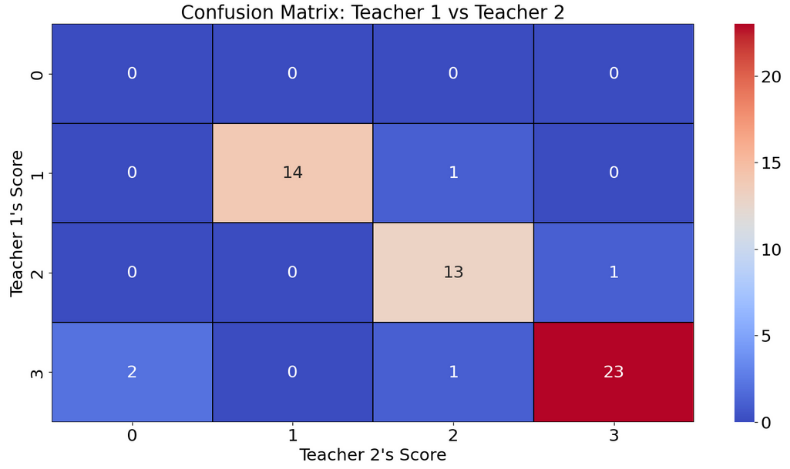
\includegraphics[width=0.7\textwidth]{agree}
    \caption{Confusion Matrix Teacher 1 compare to Teacher 2}
    \label{fig:confusion_matrices}
\end{figure}

%%%%%%%%%%%%%%%%%%%%%%%%%%%%%%%%%%%%%%%%%%%%%%%%%%%%%%%%%%%%

\section{AI vs. Human Score Comparison Tables}

An extended version of \rtab{tab:ai_human_comparison_app} 
lists per-Bloom-level Score Agreement Rate (SAR) and Cohen’s 
Kappa values. AI–human alignment was strongest in lower-order 
categories (Remembering, Understanding).

{
\setlength{\LTleft}{-0.5cm}
\setlength{\LTright}{0pt}
\centering
\begin{longtable}{l c c l}
    \caption{Detailed AI–Human Score Agreement by Bloom’s Category}
    \label{tab:ai_human_comparison_app}
    \\

    % For Header
    \hline
    \textbf{Bloom’s Level} & \textbf{SAR (\%)} & \textbf{Cohen's Kappa} & \textbf{Dominant Divergence Type} \\
    \hline
    \endfirsthead

    % For Overflow Header
    \hline
    \textbf{Bloom’s Level} & \textbf{SAR (\%)} & \textbf{Cohen's Kappa} & \textbf{Dominant Divergence Type} \\
    \hline
    \endhead

    % For Footer
    \hline
    \endfoot

    Remembering & 91.2 & 0.85 & Lexical synonym mismatch \\
    Understanding & 86.7 & 0.82 & Missing elaboration cues \\
    Applying & 81.3 & 0.77 & Ambiguous interpretation of examples \\
    Analyzing & 76.1 & 0.73 & Over-scoring detailed but incorrect logic \\
    Creating & 74.5 & 0.71 & Under-scoring creative, non-template answers \\
        
\end{longtable}
}

Representative divergences were also examined manually. 
For example, in the \textit{Creating} level, AI assigned a 
score of 2 to an original but unconventional response that 
both teachers rated 3, citing “insufficient keyword match.”

%%%%%%%%%%%%%%%%%%%%%%%%%%%%%%%%%%%%%%%%%%%%%%%%%%%%%%%%%%%%

\section{LLM Explanation Quality Examples}

A stratified subset of 200 AI-generated explanations was 
annotated by human evaluators for clarity, rubric alignment, 
and coverage of assessment criteria. 
\rtab{tab:explanation_quality} presents representative 
samples across quality levels.

{
\centering
\begin{longtable}{l p{0.8\textwidth}}
    \caption{Examples of AI Scoring Explanation Quality}
    \label{tab:explanation_quality}
    \\

    % For Header
    \hline
    \textbf{Quality Level} & \textbf{Example (Translated from Thai)} \\
    \hline
    \endfirsthead

    % For Overflow Header
    \hline
    \textbf{Quality Level} & \textbf{Example (Translated from Thai)} \\
    \hline
    \endhead

    % For Footer
    \hline
    \endfoot

    High & “The response explains both concepts correctly and connects them with appropriate terminology, matching the rubric’s full-credit description.” \\
    Medium & “Shows partial understanding; correctly defines terms but lacks complete comparison.” \\
    Low & “Mentions topic keywords without explanation; reasoning unclear and not linked to rubric.” \\

\end{longtable}
}

Overall, 87\% of explanations were rated high quality, 
9\% medium, and 4\% low.

%%%%%%%%%%%%%%%%%%%%%%%%%%%%%%%%%%%%%%%%%%%%%%%%%%%%%%%%%%%%

\section{LLM Scoring Error Categorization}

LLM scoring discrepancies were categorized into four main 
% error types. \rtab{tab:error_examples} summarizes their 
frequencies and provides representative cases.

{
\setlength{\LTleft}{-2.2cm}
\setlength{\LTright}{0pt}
\centering
\begin{longtable}{l c p{0.5\textwidth} l}
    \caption{Error Type Distribution and Illustrative Examples}
    \label{tab:error_examples}
    \\
    
    % For Header
    \hline
    \textbf{Error Type} & \textbf{Frequency (\%)} & \textbf{Description / Example} & \textbf{Bloom’s Level} \\
    \hline
    \endfirsthead

    % For Overflow Header
    \hline
    \textbf{Error Type} & \textbf{Frequency (\%)} & \textbf{Description / Example} & \textbf{Bloom’s Level} \\
    \hline
    \endhead

    % For Footer
    \hline
    \endfoot

    Under-scoring & 5.8 & AI rated 2 instead of 3 due to missing explicit keyword, despite correct reasoning. & Creating \\
    Over-scoring & 6.3 & AI gave 3 for an answer with factual inaccuracy but confident phrasing. & Analyzing \\
    Partial Credit Inconsistency & 3.4 & Similar responses received different scores due to varied sentence length. & Understanding \\
    Rubric Misinterpretation & 2.1 & Model misread rubric cue; rewarded example listing instead of explanation. & Applying \\
 
\end{longtable}
}



%\end{appendices}


% must put back tocdepth to 1, otherwise list of tables and list of figures are empty
\addtocontents{toc}{\protect\setcounter{tocdepth}{1}}


%%%%%%%%%%%%%%%%%%%%%%%%%%%%%%%%%%%%%%%%%%%%%%%%%%%%%%%%%%%%%%%%%%%%%%%%%%%%%% 
%
% Acknowledgement
% (do not edit here; instead edit the file ack.tex)
%
%%%%%%%%%%%%%%%%%%%%%%%%%%%%%%%%%%%%%%%%%%%%%%%%%%%%%%%%%%%%%%%%%%%%%%%%%%%%%% 
%\newpage

\addcontentsline{toc}{chapter}{BIOGRAPHY}
\chapter*{BIOGRAPHY}
% Use full names.

\begin{table}[h]
\begin{tabular}{p{0.3\textwidth} l}
%%============================================================================
Name & \thesisauthor \\[0cm] \\ 
%Date of Birth &&&&& \hspace*{25mm}  March 31, 1980  \\ 
Education & 2020: Bachelor of Engineering \\[0cm]\\
& (Electrical Engineering) \\[0cm]\\
& Thammasat University \\[0cm]\\
& 2024: Master of Engineering \\[0cm]\\
& (Artificial Intelligence and Internet of Things) \\[0cm]\\
& \thesisinstitute \\[0cm]\\  
& Thammasat University\\
%%============================================================================
\end{tabular}
\end{table}

\noindent
\textbf{Publications}

\begin{itemize}[label={},itemindent=-2em,leftmargin=2em]
  \setlength{\itemsep}{1pt}
  \setlength{\parskip}{1pt}
  \setlength{\parsep}{2pt}
%\begin{itemize}
\item Institute, I. , Foo, M. E. , \& Gopinath, S. C. B. (2022). Feasibility of graphene in biomedical applications. to be appear in \textit{Biomedicine \& Pharmacotherapy}.

\item Institute, I., Hanot, C. C., Choi, Y. S., Anani, T. B., Soundarrajan, D., \& David, A. E. (2015). Effects of iron-oxide nanoparticle surface chemistry on uptake kinetics and cytotoxicity in CHO- K1 cells. \textit{International Journal of Molecular Sciences, 17}(1), 226-230.

\item Institute, I., Sinervo, A., \& Arkkio, A. (2012). Modeling two-pole cage induction machine equipped with embedded force actuator. \textit{Proceedings of $10^{th}$ International Conference on Vibrations in Rotating Machinery} (pp. 765-774). New York: Woodhead Publishing.
\end{itemize}

\end{document}

